\documentclass{beamer}
\usetheme{Madrid}
\usepackage{amsfonts}
\usepackage{amsmath}
\usepackage{algorithm}
\usepackage[noend]{algpseudocode}
\usepackage{multirow}
\usepackage{appendixnumberbeamer}
\usepackage{graphicx}
\usepackage{url}
\usepackage{rotating}
\usepackage{xr}
\usepackage{xmpmulti}

\newcommand{\todo}[1]{}

\setbeamertemplate{navigation symbols}{}%remove navigation symbols

\title[SV Detection]{Detecting and Analyzing Genomic Structural Variation using Distributed Computing}
\author[Chris Whelan]{Chris Whelan}

\institute[OHSU]{Oregon Health \& Science University}

\titlegraphic{
\includegraphics[height=2cm,keepaspectratio]{ohsu-logo3.jpg}}

\begin{document}

\begin{frame}
\maketitle
\end{frame}

\begin{frame}{Outline}
  \tableofcontents
\end{frame}

\section{Genomic Structural Variations and the Contributions of this Thesis}
\begin{frame}{Outline}
  \tableofcontents[currentsection]
\end{frame}

\begin{frame}{Genomic Structural Variations}
\center
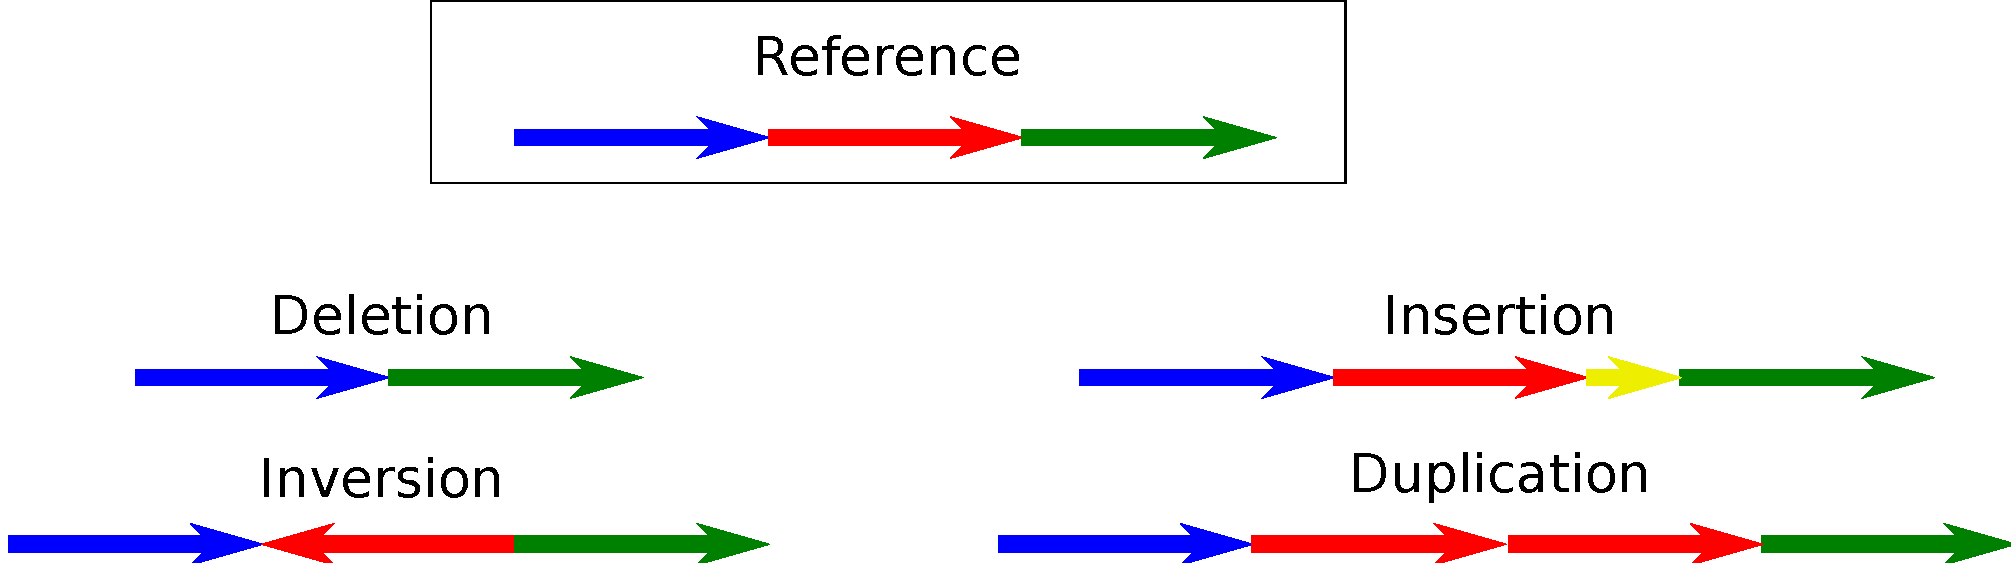
\includegraphics[width=.75\textwidth]{sv_types.pdf}
\begin{itemize}
\item Structural Variations (SVs) are differences between the genomes of individuals and the reference genome sequence that affect at least 40-50 bp of DNA
\item SV's explain most variant bases between individuals in the human
  population (Levy et al. 2007)
\item Have effects on phenotype including schizophrenia/autism, cancer-driving mutations, cardiovascular disease, likely many more
\end{itemize}
\end{frame}

\begin{frame}{Contributions of this Thesis}
\begin{itemize}
 \item Data analysis and software for determining features enriched or depleted at gibbon genome breakpoints. (Chap. 8, Carbone et al, submitted; Cappozzi et al., \emph{Genome Res.})
 \item An algorithmic framework for solving SV detection problems in Hadoop and MapReduce based on the computation of local features along the genome. (Chap. 4, RECOMB-seq 2013)
 \item Cloudbreak, an open-source Hadoop-based tool for discovering genomic deletions and insertions, which improves accuracy and achieves dramatically faster runtimes over existing approaches. (Chap. 5 \& 6, RECOMB-seq 2013)
 \item A demonstration of the combination of Cloudbreak's local feature model with a statistical sequence labelling technique (conditional random fields) to integrate multiple data sources and improve breakpoint resolution. (Chap. 7)
\end{itemize}
\end{frame}

\section{Gibbon Genome Breakpoint Analysis}
\begin{frame}{Outline}
  \tableofcontents[currentsection]
\end{frame}

\begin{frame}{Mechanisms and Scales of SV Formation}
How do SVs happen? Many mechanisms, including:
\begin{center}
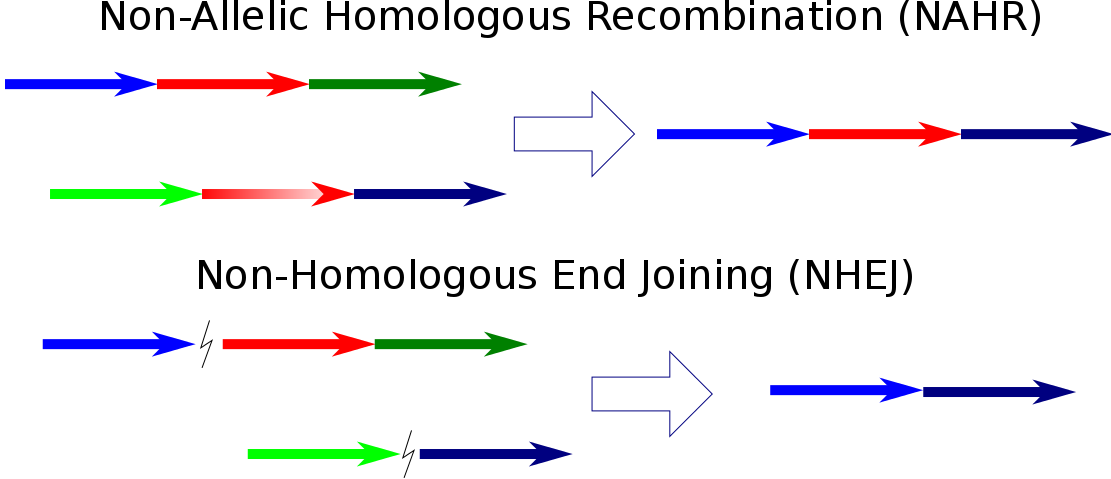
\includegraphics[width=.75\textwidth]{NAHR_NHEJ.png} \\
% \begin{itemize}
% \item Non-allelic Homologous Recombination (NAHR)
% \item Non-homologous End Joining (NEHJ)
% \item Mobile Element Insertion (MEI)
% \end{itemize} 
\end{center}
SVs can be present at different population scales
\begin{itemize}
  \item Cells in a tumor (somatic mutations)
  \item Individuals in a population
  \item Between the genomes of different species
\end{itemize}
\end{frame}


\begin{frame}{SVs in the Gibbon Genome}
What can we infer about SV formation mechanisms and timing in a primate genome heavily rearranged by SVs?
\begin{itemize}
  \item Gibbons have very different karyotypes from the rest of the apes
  \item Search for enriched sequence features near evolutionary breakpoints
  \item Monte Carlo based location permutation approach
     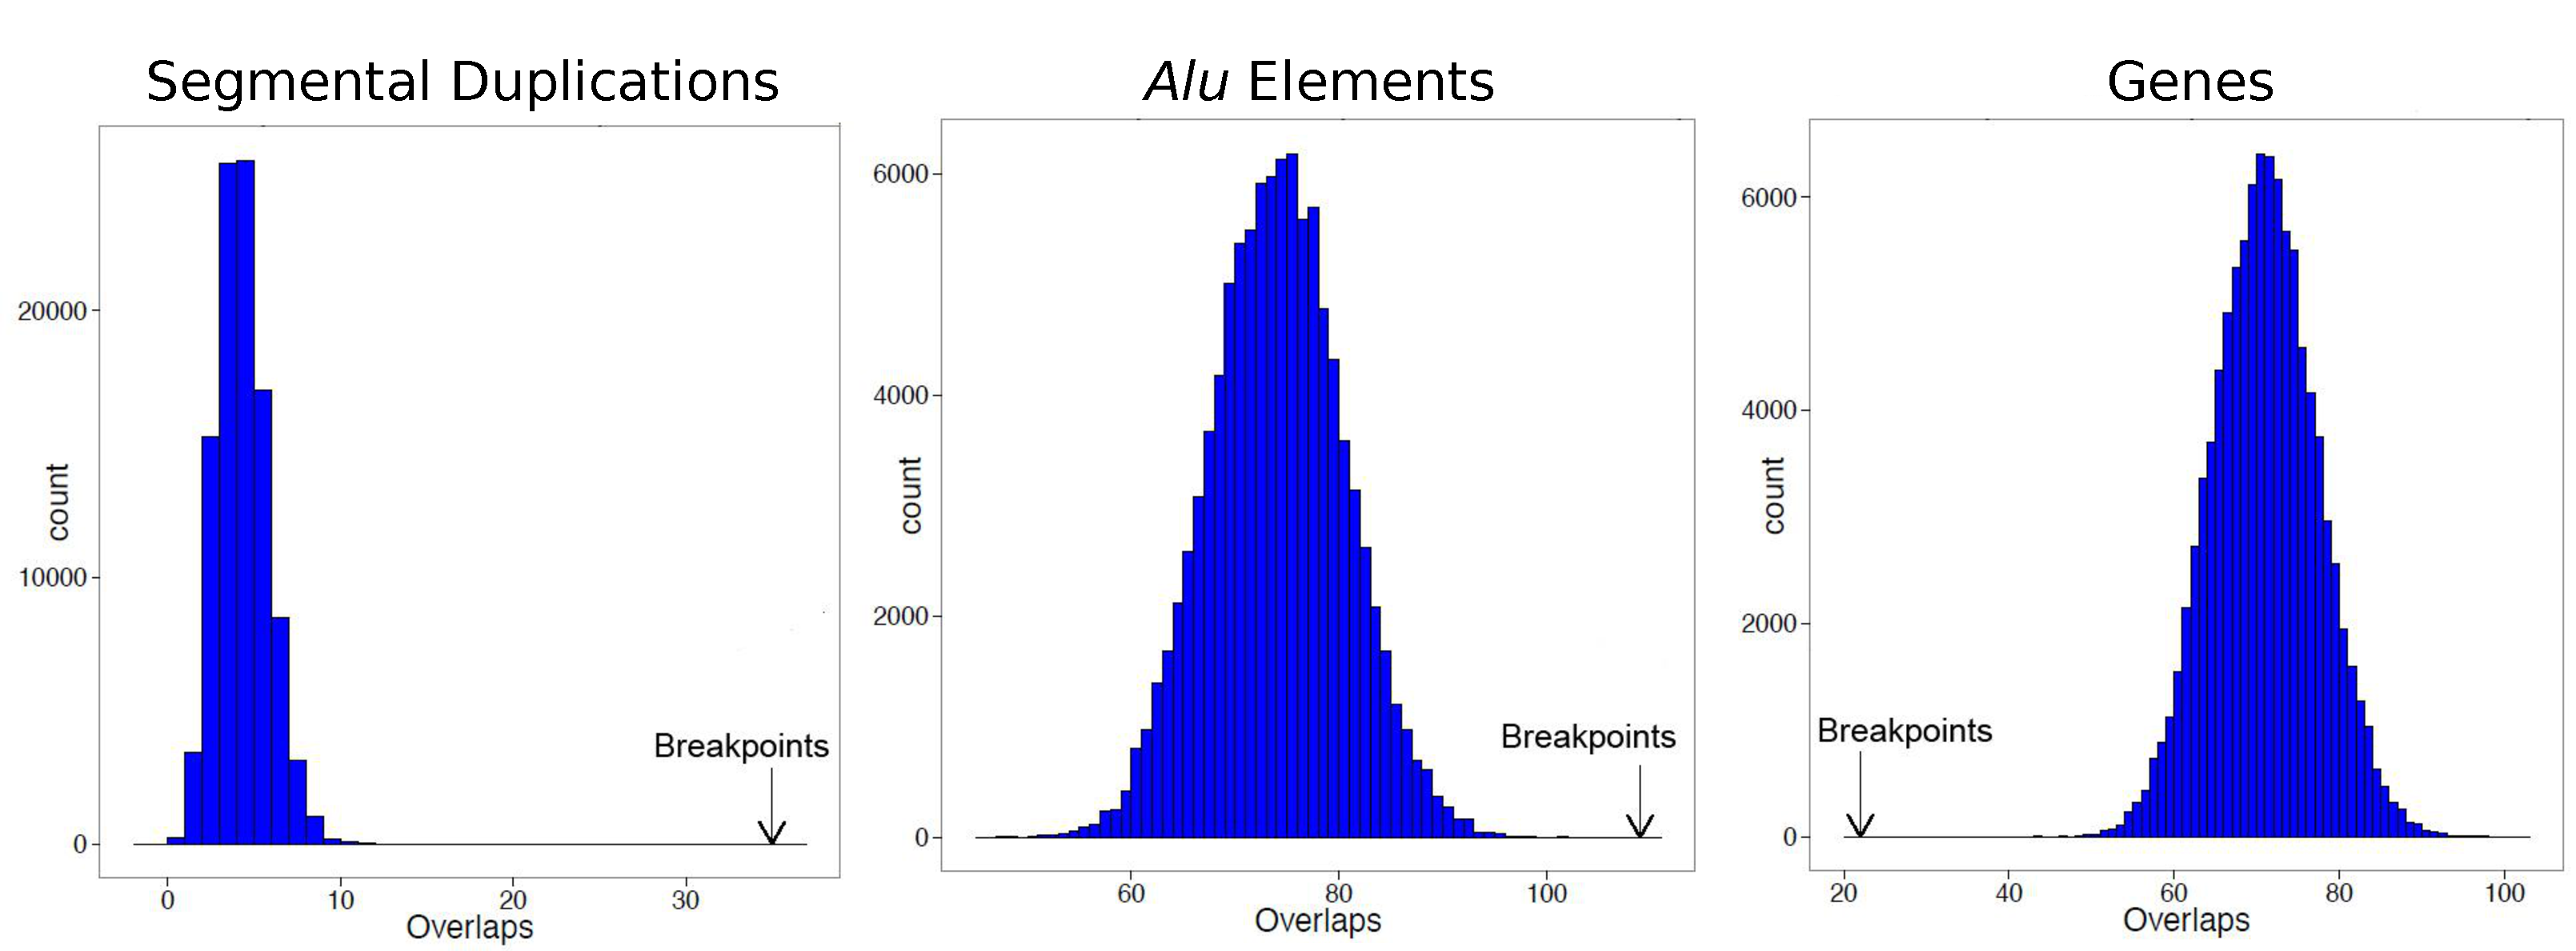
\includegraphics[width=.75\textwidth]{gibbon_genome_histograms.pdf}
  \item Run tests, distribute permutations over cluster with Condor: \\
  \small  \url{https://github.com/cwhelan/permuting-feature-enrichment-test}
\end{itemize}
\end{frame}

\section{Detecting SVs from Short-Read Sequencing Data}
\begin{frame}{Outline}
  \tableofcontents[currentsection]
\end{frame}

\begin{frame}{Short-Read Data for Resequencing}
\center
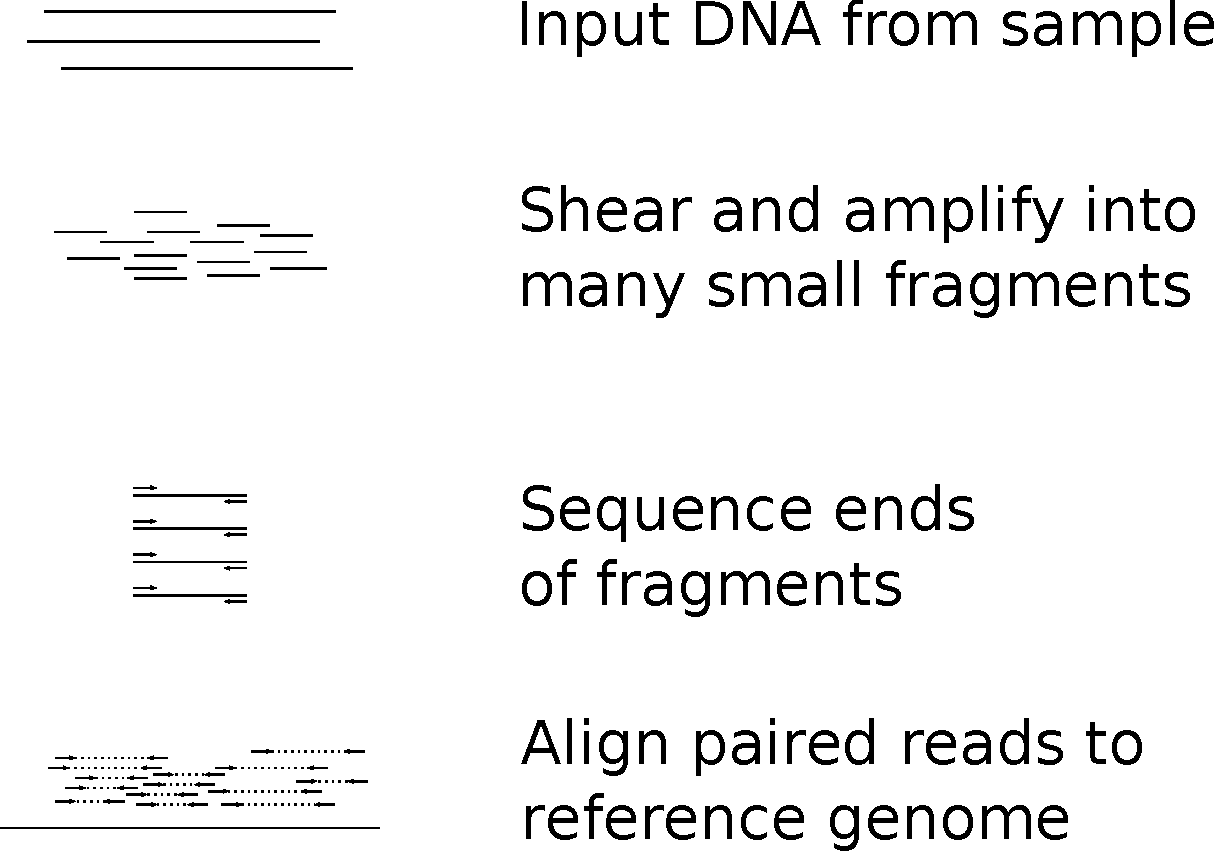
\includegraphics[width=.75\textwidth]{short_read_sequencing.pdf}
\end{frame}

\begin{frame}{SV Detection from Short-Read Sequencing Data}
\begin{itemize}
  \item Multiple signals of SVs in short read sequencing data
  \item Read-pair (RP) detection most commonly used
\begin{center}
     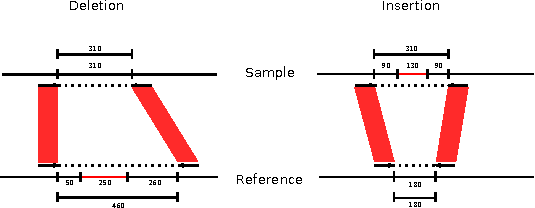
\includegraphics[height=.3\textheight]{rp_signatures_opaque.pdf}
\end{center}
  \item Read depth (RD), Split-Read (SR), Assembly (AS)
\vspace{1mm}
\begin{center}
     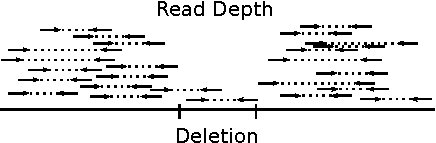
\includegraphics[width=.4\textwidth]{rd.pdf}\hspace{2mm}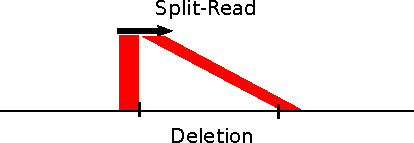
\includegraphics[width=.4\textwidth]{sr.pdf}
\end{center}
\end{itemize}
\end{frame}

% \begin{frame}{SV detection is hard}
% \begin{itemize}
% \item Large number of methods
% \item Limited concordance between methods, low sensitivity and
%   specificity 
% \item Some variant classes are difficult to detect (i.e. 100bp deletions)
% \end{itemize}
%  \begin{center}
%      \includegraphics[height=0.5\textheight]{/users/cwhelan/Documents/gene_rearrange/svpipeline/MillsDeletionDiscoverySensitivtyAndFDR.png}
%    \end{center}
% \fontsize{7.5pt}{10}\selectfont
% \hfill 
%    Mills et al. 2011
% \end{frame}

\begin{frame}{Read-pair approaches extend to consider more data}
The Traditional Approach:
 \begin{center}
     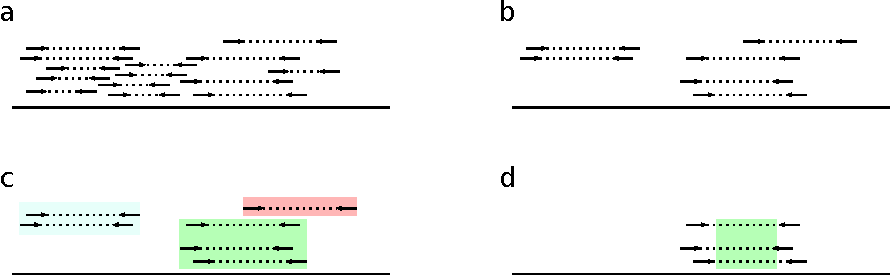
\includegraphics[width=0.6\textwidth]{rp_method_workflow.pdf}
   \end{center}
\fontsize{10pt}{10}\selectfont
\begin{itemize}
\item Multiply-mapped read pairs
\begin{itemize}
\item MrFAST - Hormozdiari et al (2009), HYDRA - Quinlan et al. (2010), GASVPro - Sindi et al. (2012)
\end{itemize}
\item Concordant read pairs (Read depth signals, smaller variations)
\begin{itemize}
\item GASVPro, CLEVER - Marschall et al. (2012)
\end{itemize}
\item Split read signals
\begin{itemize}
\item DELLY - Rausch et al (2012)
\end{itemize}
\item All of the above + population-scale signals
\begin{itemize}
\item Genome STRiP - Handsaker et al. (2011)
\end{itemize}
\item Computational requirements increase with the amount of data examined
\item How can we scale algorithms to new data sizes?
\end{itemize}
\end{frame}

\begin{frame}{The amount of sequencing data is growing exponentially}
\begin{center}
  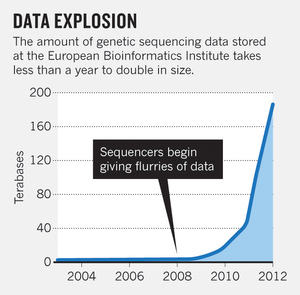
\includegraphics[width=0.3\textwidth]{ebi_data_explosion.jpg}\hspace{1mm} 
  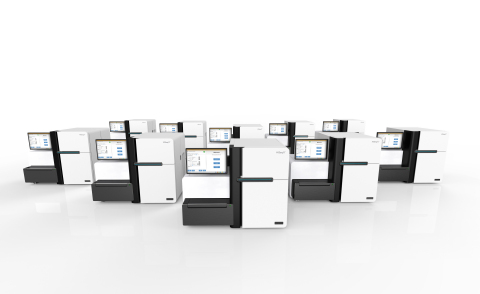
\includegraphics[width=0.5\textwidth]{HiSeqX_Ten_Image.jpg}
  
\end{center}
\begin{itemize}
  \item For large scale research projects and eventual clinical applications, need to improve analysis throughput and latency
  \item Lots of recent efforts to shorten analysis pipelines (alignment and SNV calling)
  \item Structural variation detection can be left behind
\end{itemize}
\end{frame}


%4 MapReduce framework
\begin{frame}{The MapReduce distributed computing framework}
  \begin{columns}
\column{.6\textwidth}
  \begin{itemize}
  \item Created at Google for web-scale data (Dean and
    Gehemewat 2008)
  \item Open source Hadoop implementation
  \item Used by the web giants
  \item Distributes big data sets across cluster
  \item Provides a framework for parallelization
  \item Used in bioinformatics for:
  \begin{itemize}
    \item Alignment/SNP calling (Crossbow - Langmead 2009)
    \item RNA-seq (Myrna - Langmead 2010)
  \end{itemize}
 \end{itemize}
\column{.4\textwidth}
    
\includegraphics[width=.7\textwidth]{hadoop_user_logos.pdf}
%    \vspace{10mm}
%    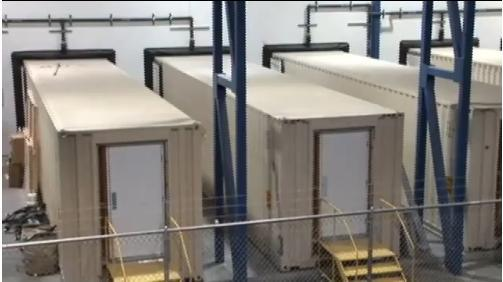
\includegraphics[width=.8\textwidth]{google-server-container.jpg}
\end{columns}
\end{frame}


\begin{frame}{Hadoop/MapReduce is not just a job scheduler}  
  \begin{columns}
    \column{.4\textwidth}
    Why not just distribute with a file server and a grid scheduler?
      \begin{itemize}
        \item<2-> Automatic redundancy of data
        \item<3-> Takes into account data locality
        \item<4-> Can handle failure of data or workers transparently
        \item<5-> Can scale linearly with the amount of data, number of nodes
      \end{itemize}
    \column{.6\textwidth}
%     \only<4>{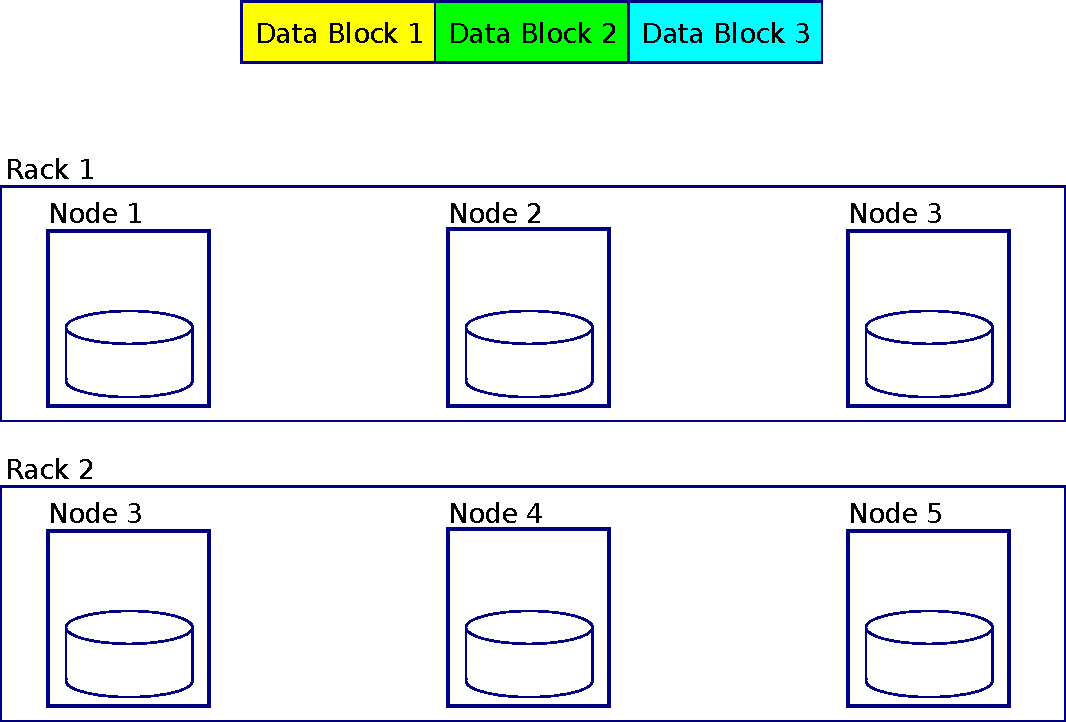
\includegraphics[scale=0.4]{hadoop_benefits_base.pdf}}
%     \onslide<2>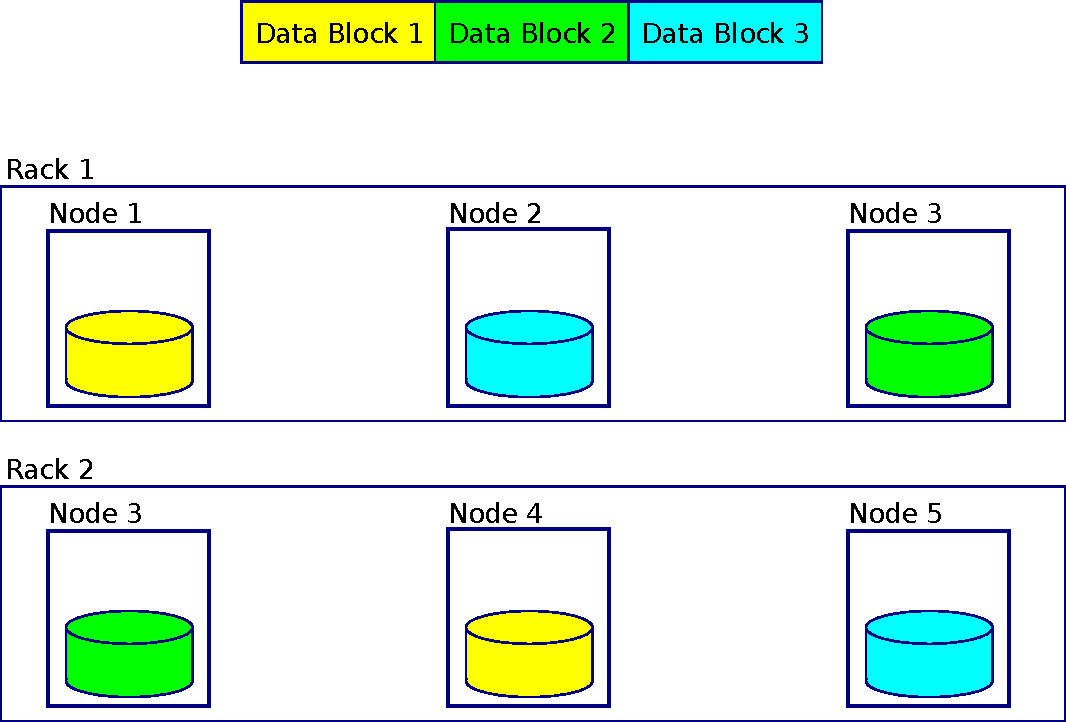
\includegraphics[width=\textwidth]{hadoop_benefits_redundant_data.pdf}
    % \onslide<3>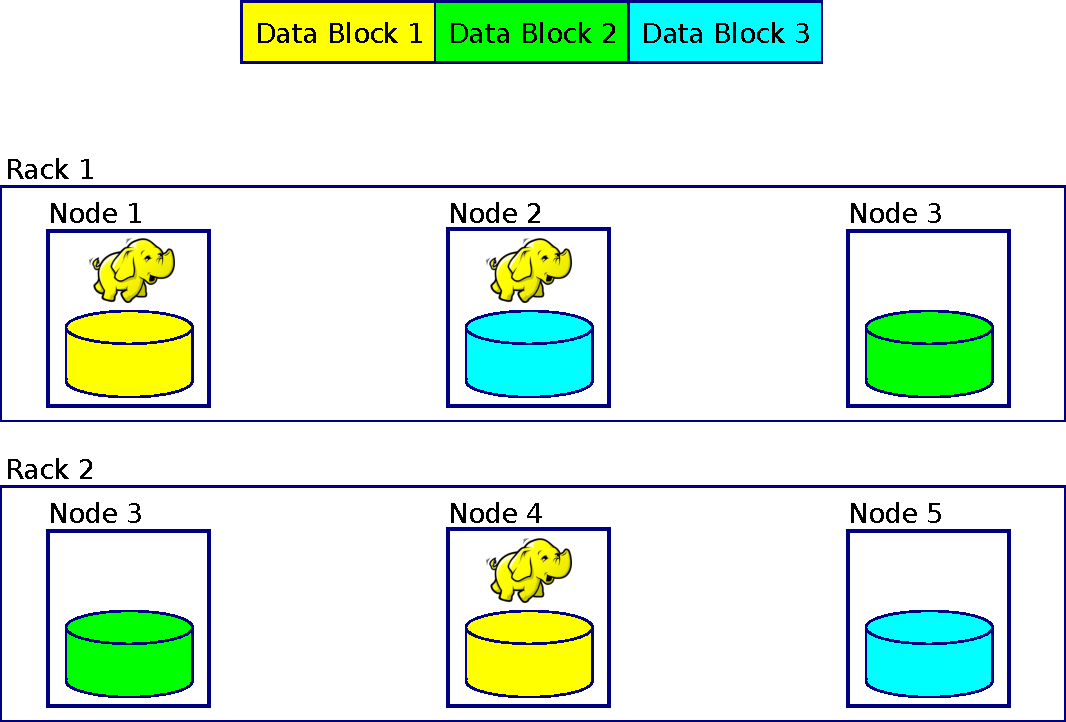
\includegraphics[width=\textwidth]{hadoop_benefits_data_locality.pdf}
    % \onslide<4>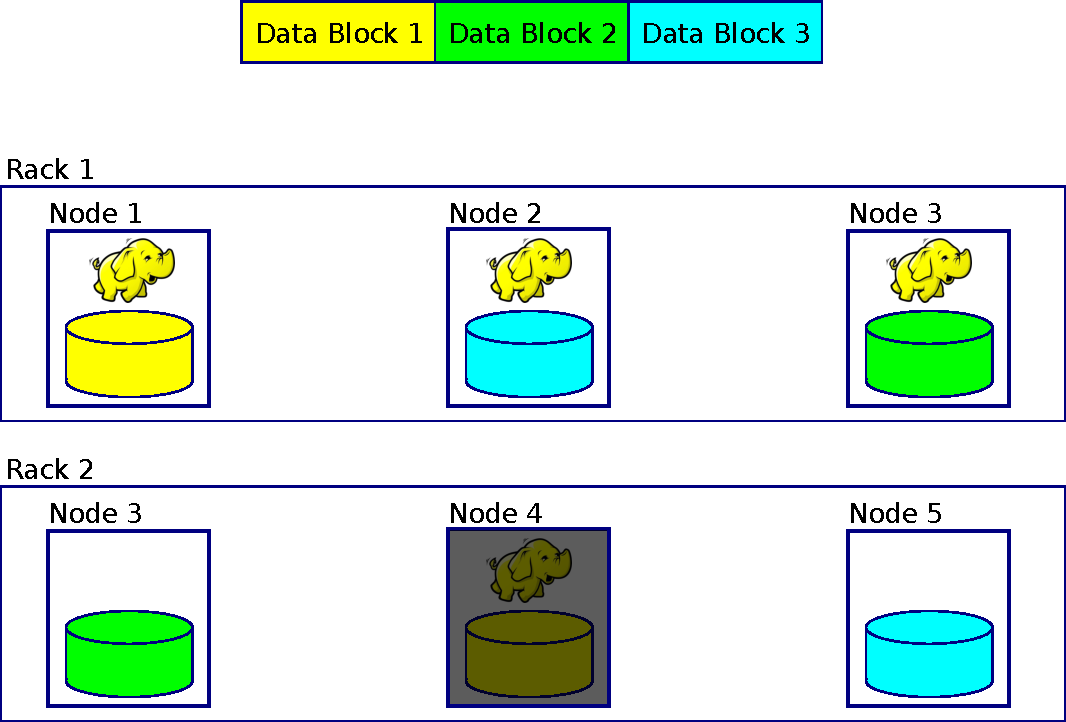
\includegraphics[width=\textwidth]{hadoop_benefits_failover.pdf}
\begin{figure}
  \centering
     \multiinclude[<+->][format=png,graphics={width=\textwidth}]{hadoop_benefits}
\end{figure}
 \end{columns}
\end{frame}

\begin{frame}{Developing algorithms in MapReduce}
  \begin{itemize}
  \item To get these properties there are constraints on application developers
  \item MapReduce divides execution into \emph{Map} and \emph{Reduce} tasks
  \end{itemize}
  \begin{center}
    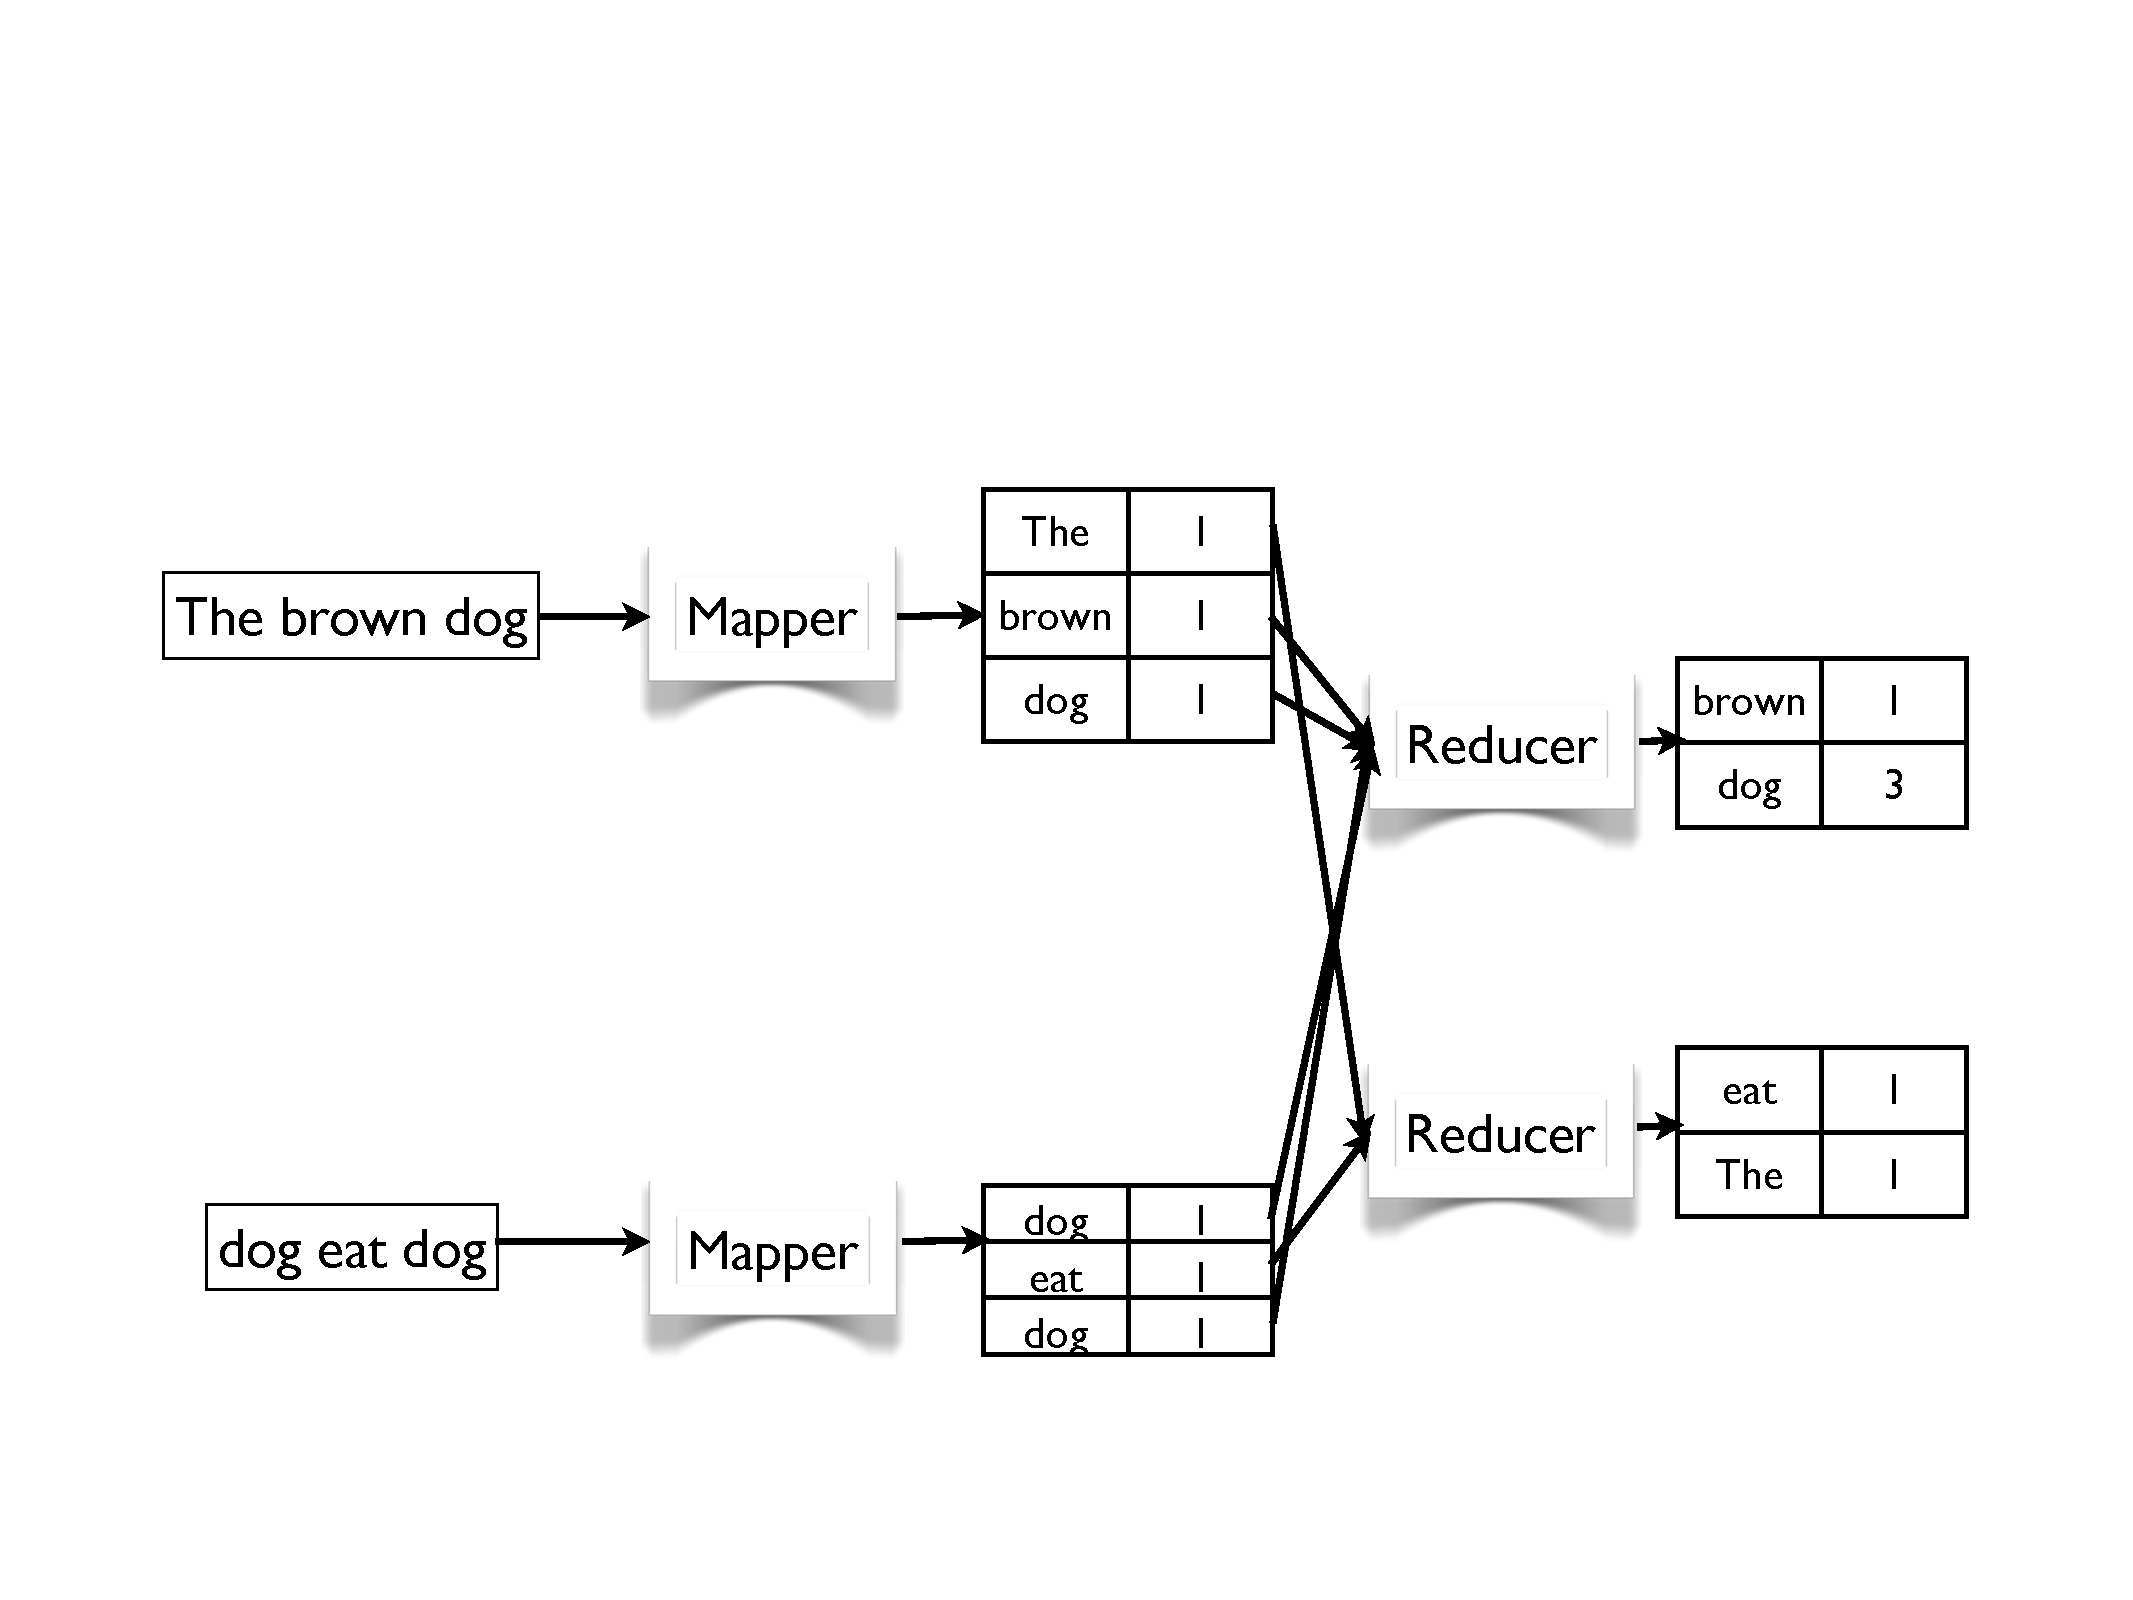
\includegraphics[trim=0 100 0 200, clip, width=\textwidth,height=0.52\textheight,keepaspectratio]{mapreduce_example.pdf}
   \end{center}
   \begin{itemize}
     \item Need to design algorithms that run independent calculations on small chunks of data
     \item How can we implement SV calling in this framework?
   \end{itemize}
\end{frame}


\section{Cloudbreak: Applying Distributed Computing to SV Detection}
\begin{frame}{Outline}
  \tableofcontents[currentsection]
\end{frame}

% \begin{frame}{SV Detection in MapReduce}
%   \begin{itemize}
%     \item Clustering of read pairs as in traditional RP algorithms
%       typically involves global compuations or graph structures
%     \item MapReduce, on the other hand, forces local, parallel
%       computations
%     \item Our approach: use MapReduce to compute features for each
%       location in the genome from alignments relevant to that location
%     \item Locations can be small tiled windows to make the problem
%       more tractable
%     \item Make SV calls from features computed along the genome in a
%       post-processing step
%   \end{itemize}
% \end{frame}

\begin{frame}{Computing local features enables parallelization}
\begin{center}
\only<1>{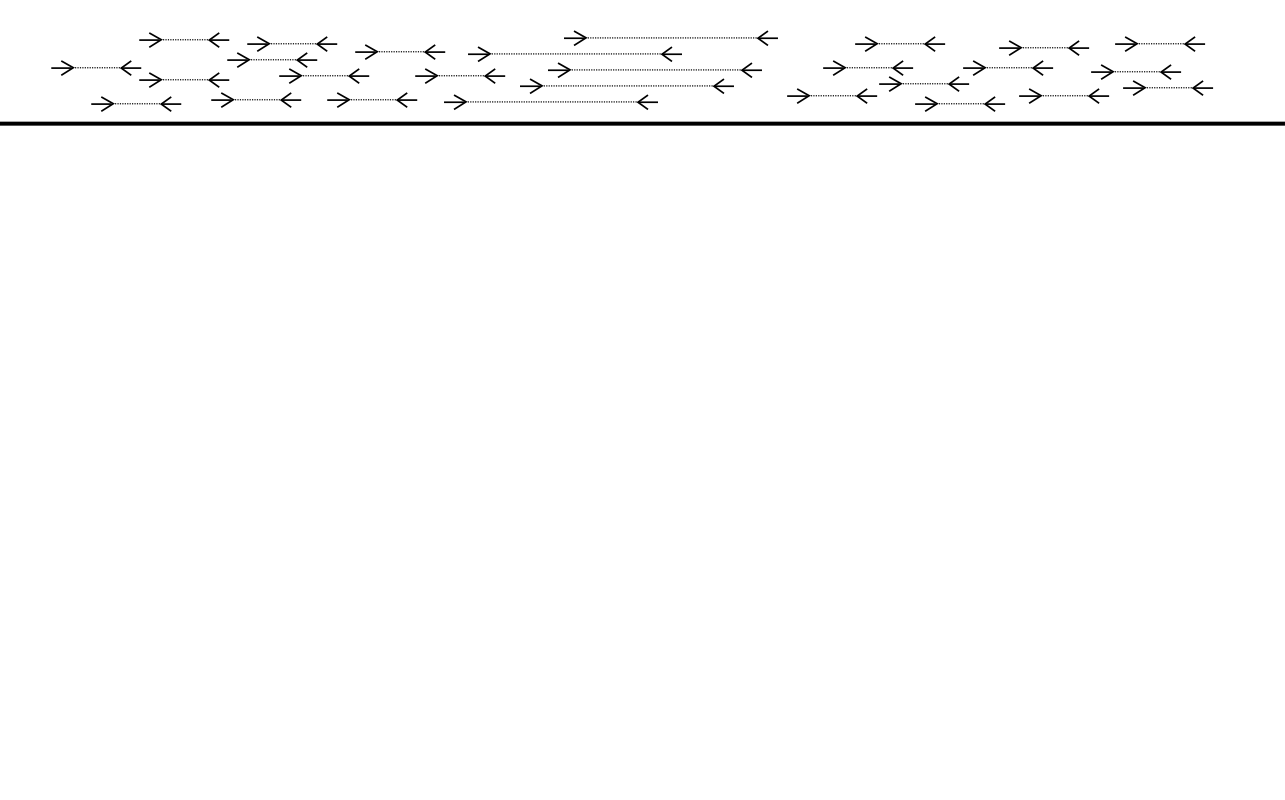
\includegraphics[height=0.8\textheight,keepaspectratio]{read_pairs_mapped.png}}
\only<2>{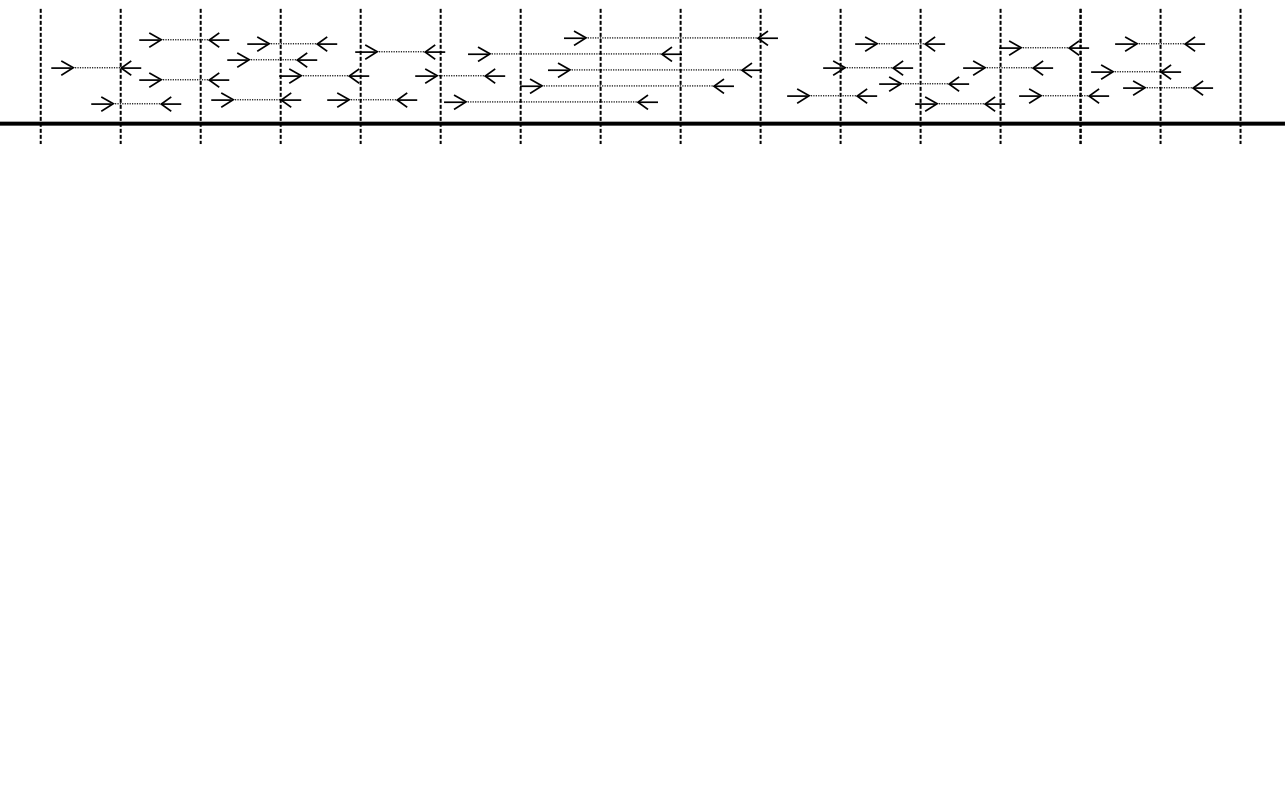
\includegraphics[height=0.8\textheight,keepaspectratio]{read_pairs_mapped_with_windows.png}}
\only<3>{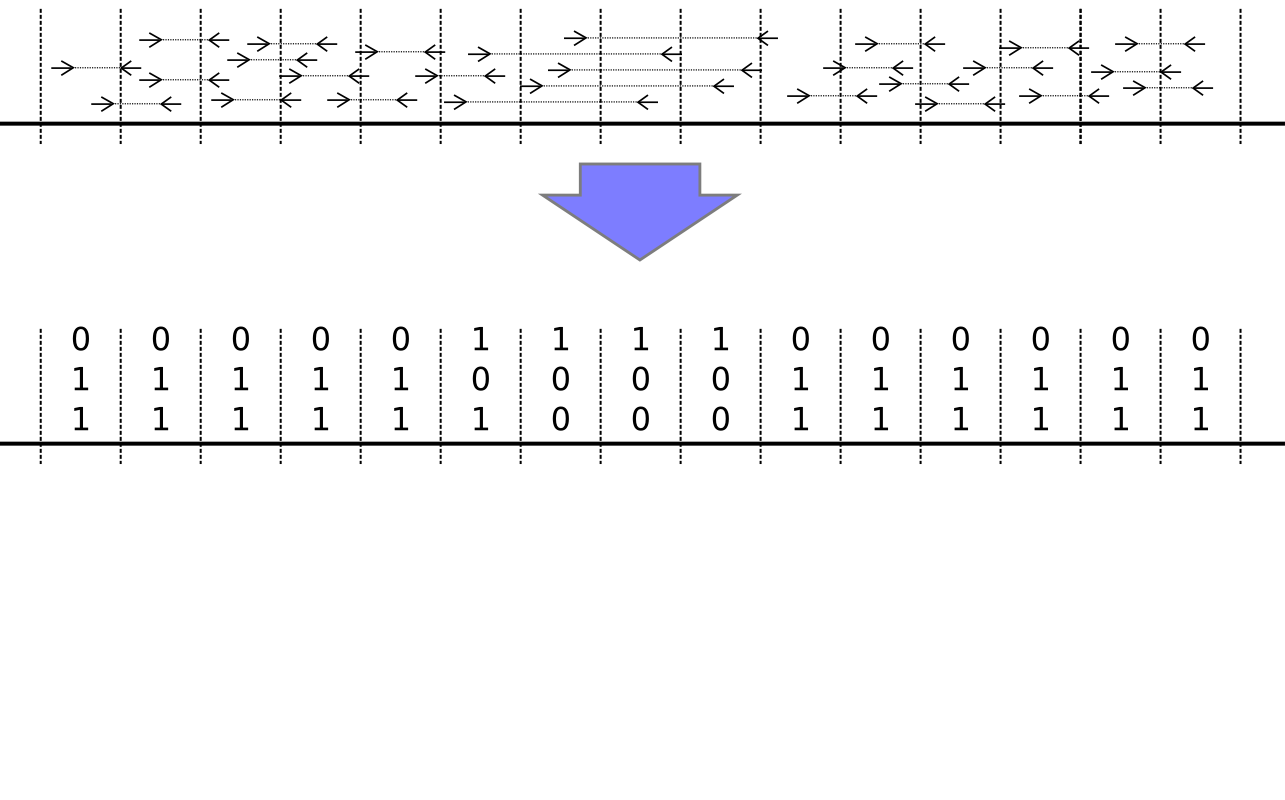
\includegraphics[height=0.8\textheight,keepaspectratio]{read_pairs_mapped_with_windows_and_features.png}}
\only<4>{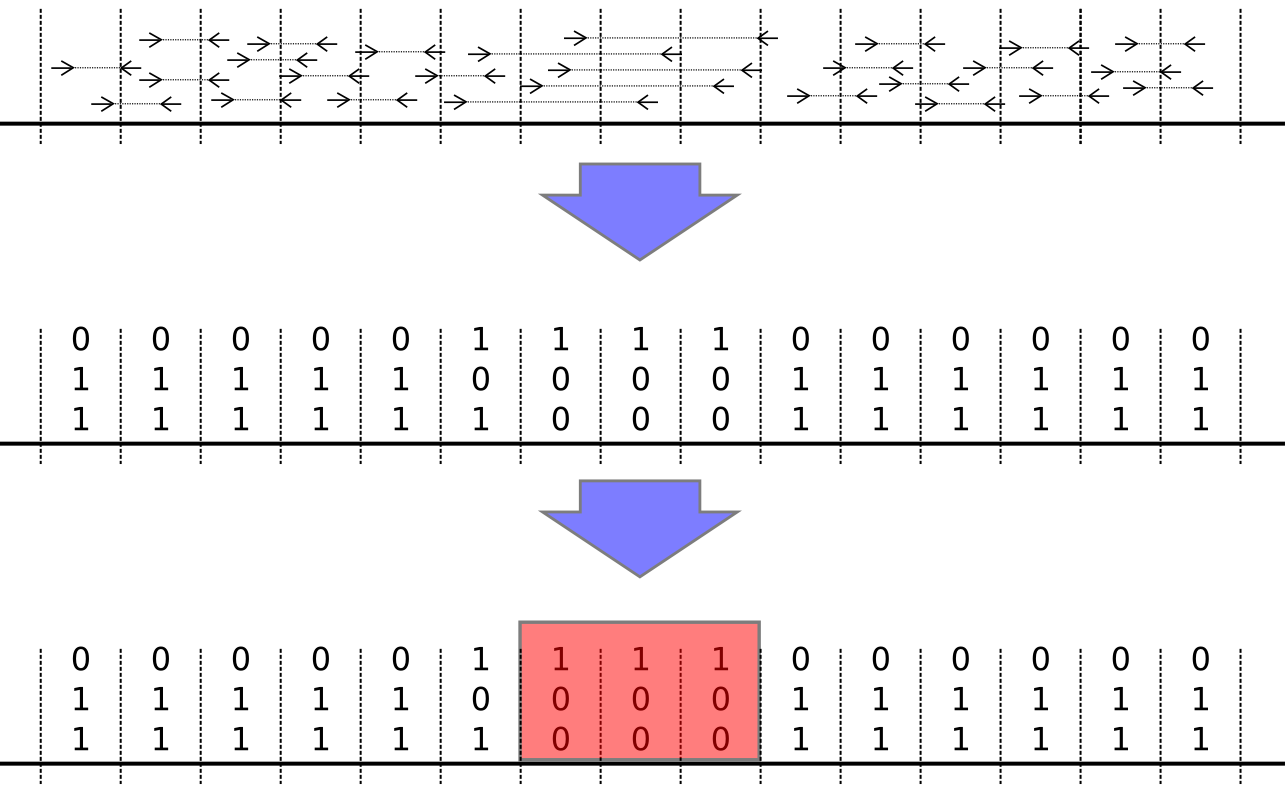
\includegraphics[height=0.8\textheight,keepaspectratio]{read_pairs_mapped_with_windows_and_features_and_call.png}}
\end{center}
\end{frame}

% 5 Cloudbreak overview (3 jobs)
% \begin{frame}{Three user-defined functions}
%   \begin{itemize}
%     \item This framework leaves three functions to be defined
%     \item May be many different approaches to take within this
%       framework, depending on the application
%   \end{itemize}
% \begin{flalign*}
%  \textsc{Loci} :& \langle a_{1},a_{2} \rangle \rightarrow L_m \subseteq L \\
%  \Phi :& \left\{\mathrm{ReadPairInfo}\;rpi_{m,i,j}\right\} \rightarrow \mathbb{R}^N \\
%  \textsc{PostProcess} :& \left\{\phi_1,\phi_2,\ldots,\phi_N\right\} \rightarrow \left\{\langle  \mathrm{SVType}\;s, l_{start}, l_{end} \rangle\right\} 
% \end{flalign*}
% \end{frame}

% \begin{frame}{Cloudbreak implementation}
%   \begin{itemize}
%   \item We focus on detecting deletions and small insertions
%   \item Implemented as a native Hadoop application
%   \item Use features computed from fitting a mixture model to the
%     observed distribution of insert sizes at each locus
%   \item Process as many mappings as possible for ambiguously mapped reads
%   \end{itemize}
% \end{frame}


% \begin{frame}{A framework for SV Detection in MapReduce}
%   \begin{center}
%     \includegraphics[width=\textwidth,height=0.9\textheight,keepaspectratio]{/users/cwhelan/Documents/svpipeline/manuscript/diagrams/workflow.png}
%    \end{center}
% \end{frame}

% 9 Mixture of distributions
\begin{frame}{Mixture of distributions provides local features}
  \begin{center}   
    \only<1>{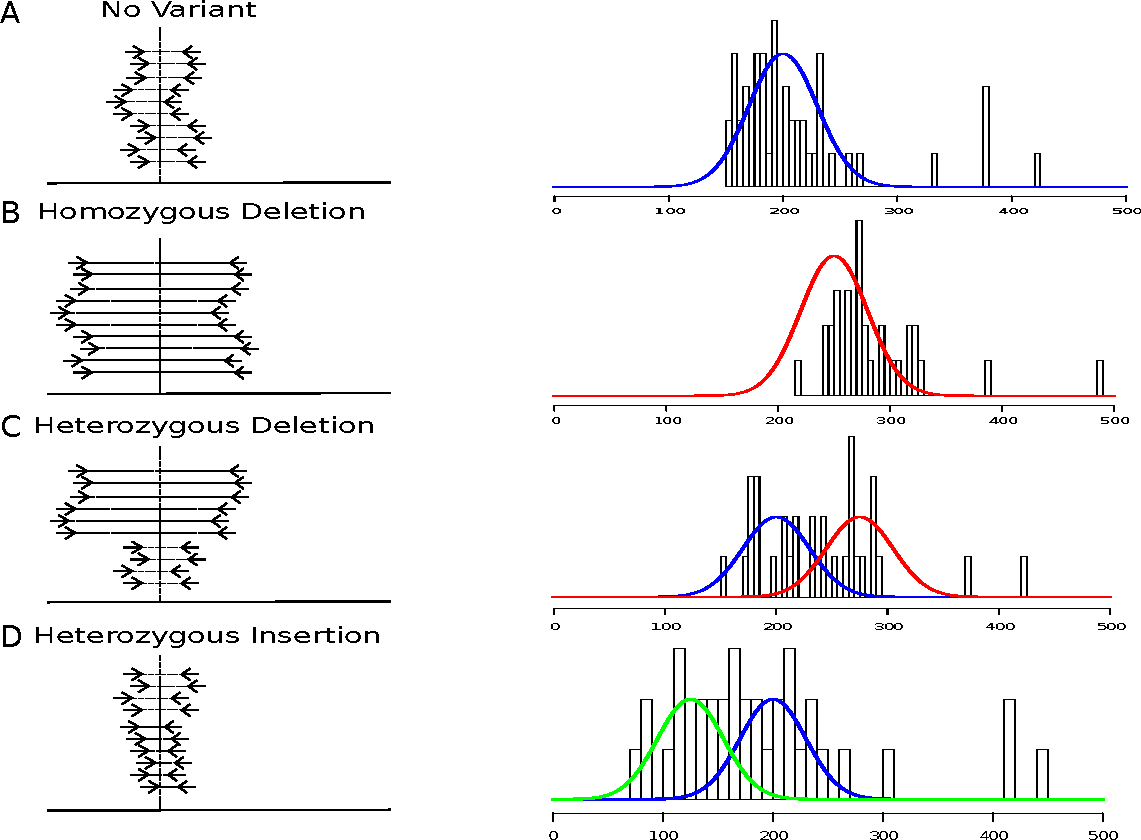
\includegraphics[trim=0 0 0 0, clip,
      height=0.5\textheight,keepaspectratio]{insert_size_mixtures.pdf}}
    \only<2>{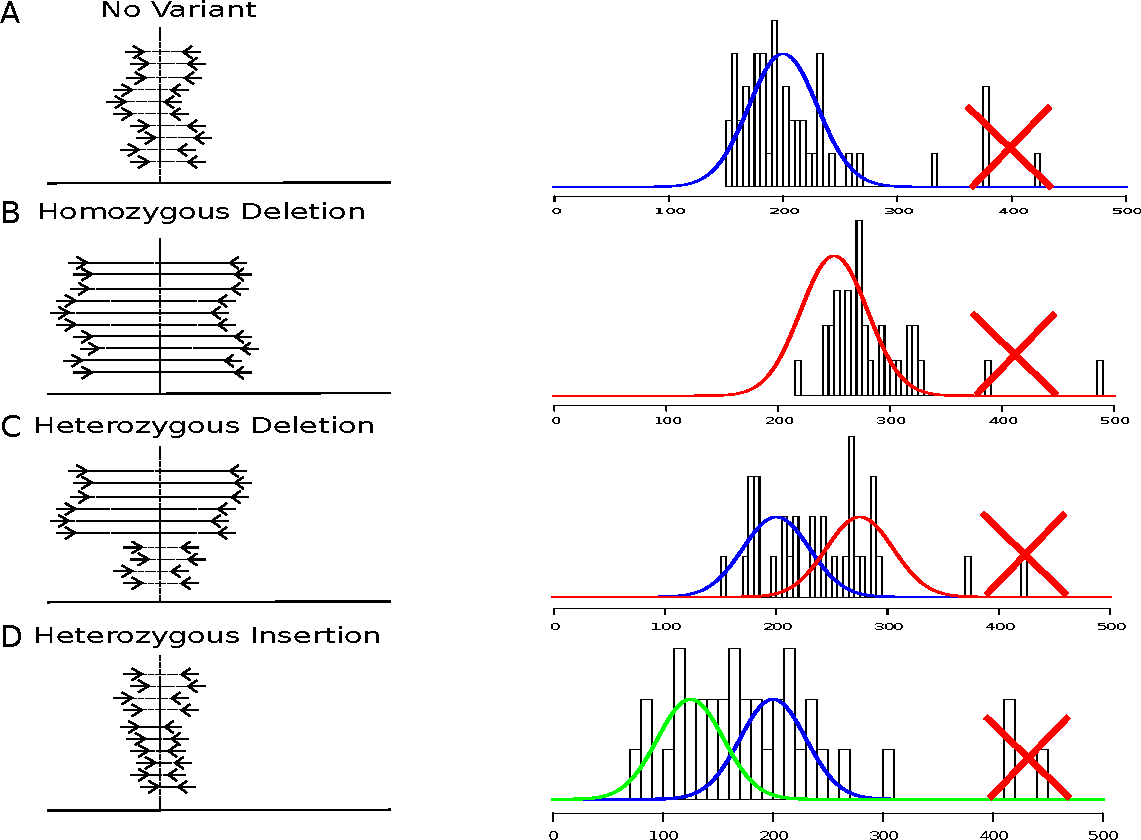
\includegraphics[trim=0 0 0 0, clip, height=0.5\textheight,keepaspectratio]{insert_size_mixtures_noise_reduction.pdf}}
  \end{center}
\begin{itemize}
\item Single sample, insertions and deletions (40bp - 25kb)
\item General idea first proposed by MoDIL (Lee et al. 2009)
\item Fit a Gaussian Mixture Model and generate features:
\begin{itemize}
 \item LR: likelihood ratio of two-component model to no-variant model
 \item $\mu'$: estimated mean of second component
 \item $\alpha$: estimated mixing weight of two components
\end{itemize}
\end{itemize}
\end{frame}

% \begin{frame}{Local distributions of insert sizes}
%   \begin{itemize}
%   \item Estimate distribution of insert sizes observed at each window
%     as a Gaussian mixture model (GMM)
%   \item Similar to idea in MoDIL (Lee et al. 2009)
%   \item Use a constrained expectation-maximization algorithm to find
%     mean, weight of second component. Constrain one component to have the
%     library mean insert size, and constrain both components to have
%     the same variance. Find mean and weight of the second component.
%   \item Features computed include the log likelihood ratio of fit
%     two-component model to the likelihood of the insert sizes under a
%     model with no variant: normal distribution under library
%     parameters.
%   \item Other features: weight of the second component, estimated mean
%     of the second component.
%   \end{itemize}
% \end{frame}

% \begin{frame}{Handling ambiguous mappings}
%   \begin{itemize}
%   \item Incorrect mappings of read pairs are unlikely to form clusters of insert sizes at a given window
%   \item Before fitting GMM, remove outliers using a nearest neighbor
%     method: If $k$th nearest neighbor of each mapped pair is greater
%     than c * (library fragment size SD) away, remove that mapping
%   \item Control number of mappings based on an adaptive cutoff for
%     alignment score: Discard mapping m if the ratio of the best
%     alignment score for that window to the score of m is larger than
%     some cutoff. This allows visibility into regions where no reads
%     are mapped unambiguously.
%   \end{itemize}
% \end{frame}

% \begin{frame}
%   \frametitle{Postprocessing}
%   \begin{itemize}
%     \item First extract contiguous genomic loci where the
%       log-likelihood ratio of the two models is greater than a given
%       threshold.
%     \item To eliminate noise we apply a median filter with window size
%       5.
%     \item Let $\mu'$ be the estimated mean of the second component and
%       $\mu$ be the library insert size. We end regions when $\mu'$
%       changes by more than 60bp ($2\sigma$), and discard regions where the length of the region differs from
%       $\mu'$ by more than $\mu$.
%     \item Cloudbreak looses some resolution to breakpoint location
%       based on genome windows and filters.
%   \end{itemize}
% \end{frame}

\begin{frame}{Cloudbreak output example}
  \begin{center}   
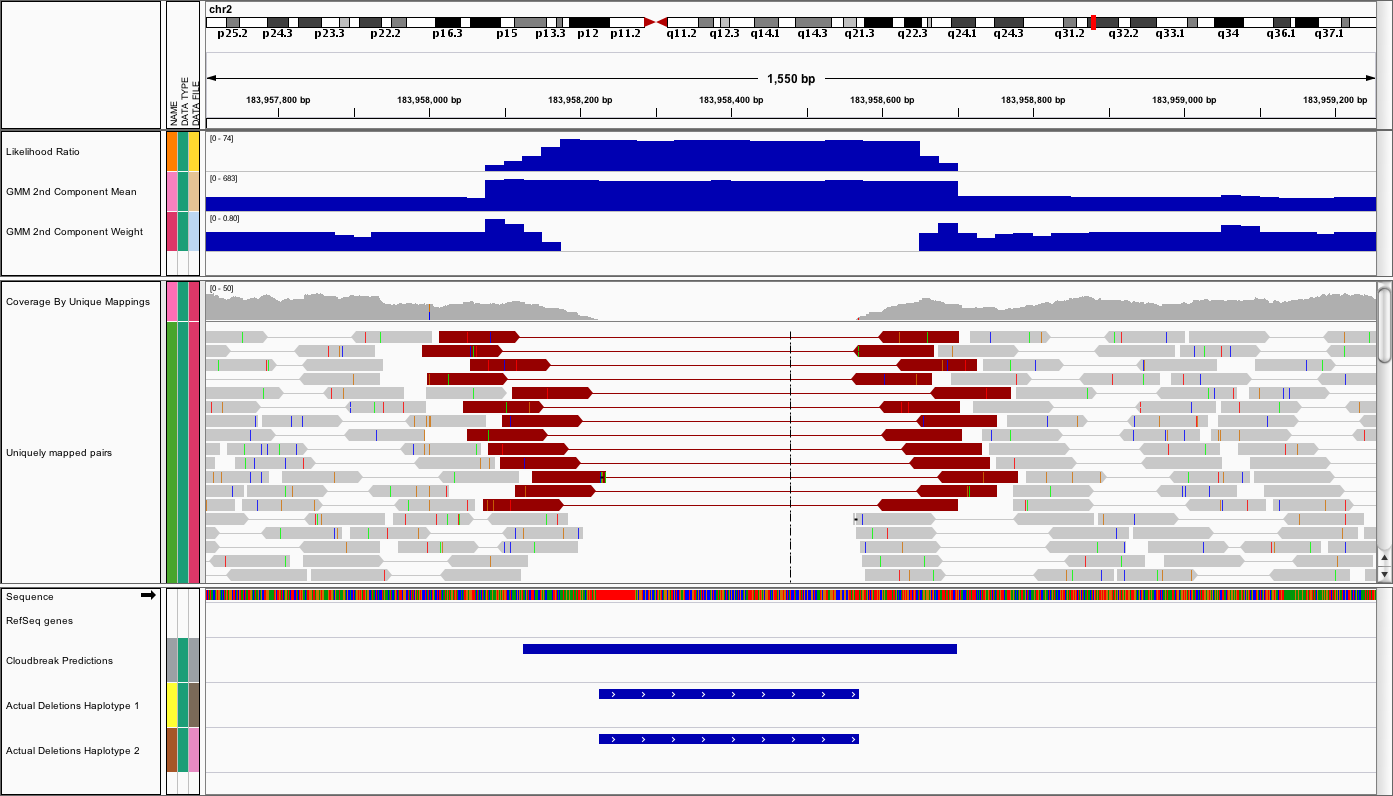
\includegraphics[width=\textwidth,height=0.8\textheight,keepaspectratio]{Cloudbreak_deletion_example.png}
  \end{center}  
\end{frame}

% 6 Algo part 1 - mapping
\begin{frame}{Cloudbreak Algorithm Job 1: Alignment}
  \begin{center}   
    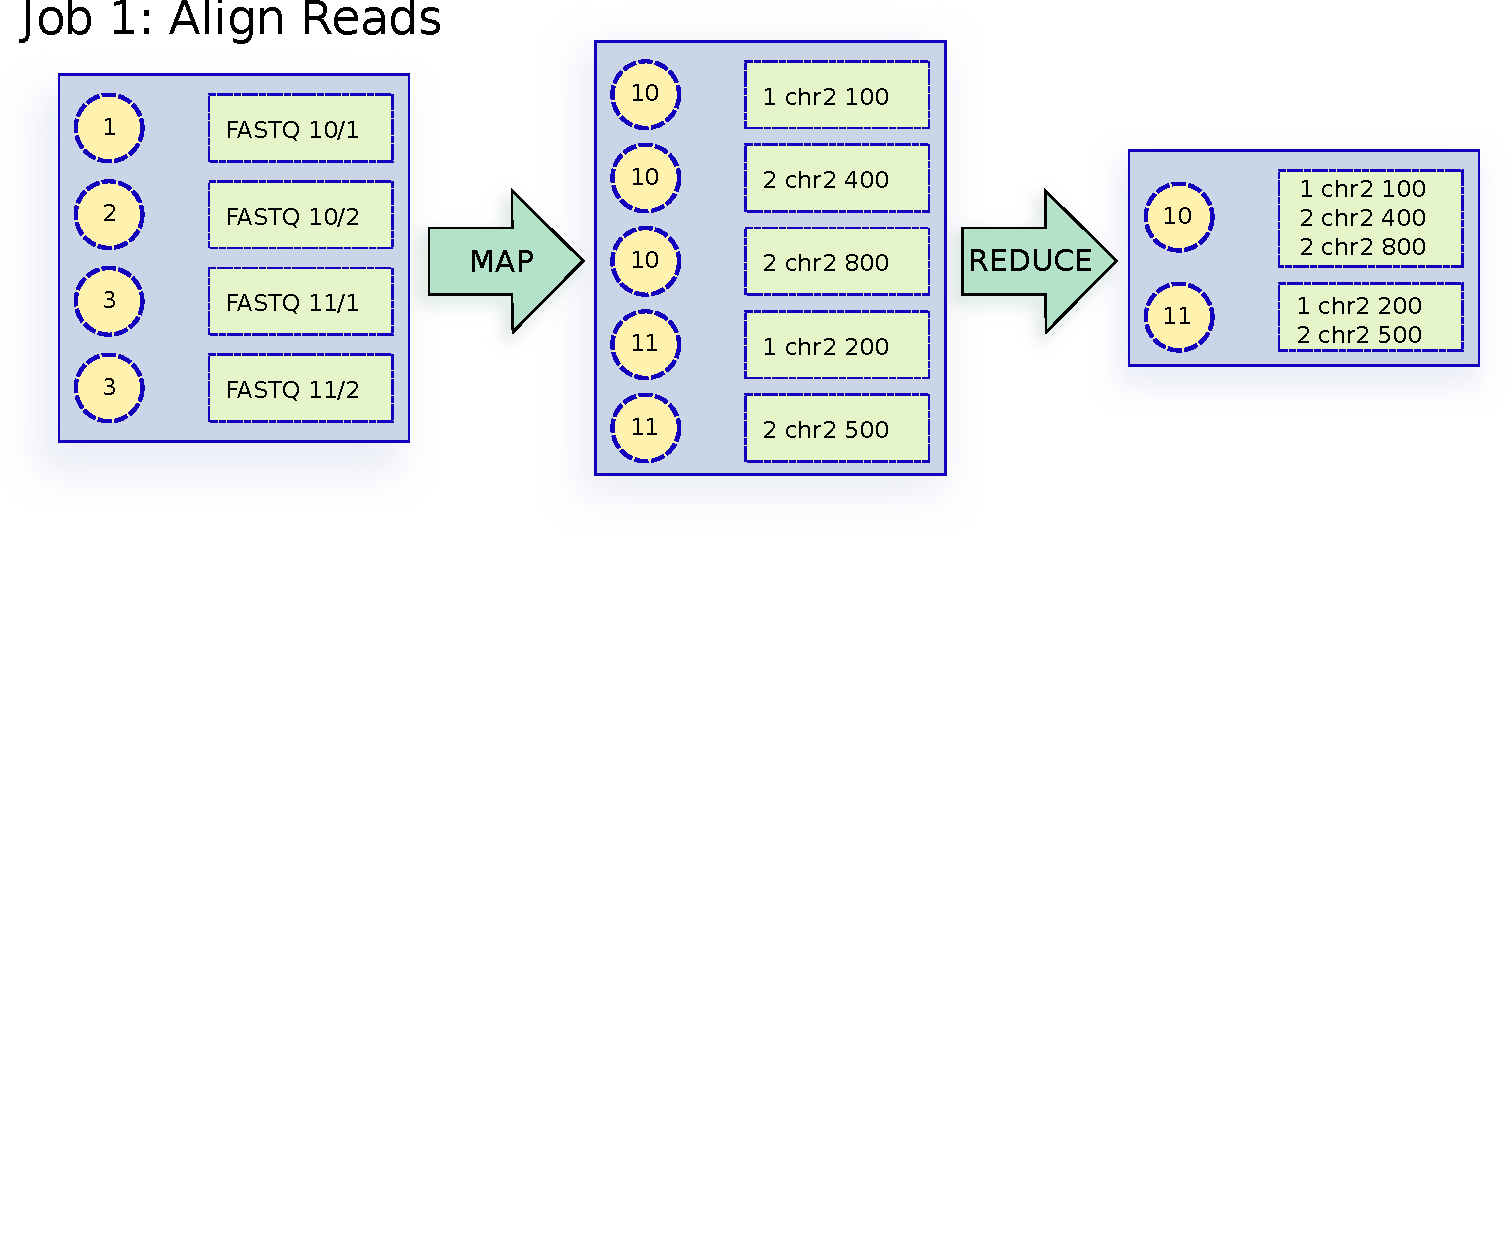
\includegraphics[width=\textwidth,height=0.8\textheight,keepaspectratio]{cloudbreak_mapred_diagram_build_1.pdf}
  \end{center}
\end{frame}


%7 Algo part 2 - features
\begin{frame}{Cloudbreak Algorithm Job 2: Compute Features}
  \begin{center}   
    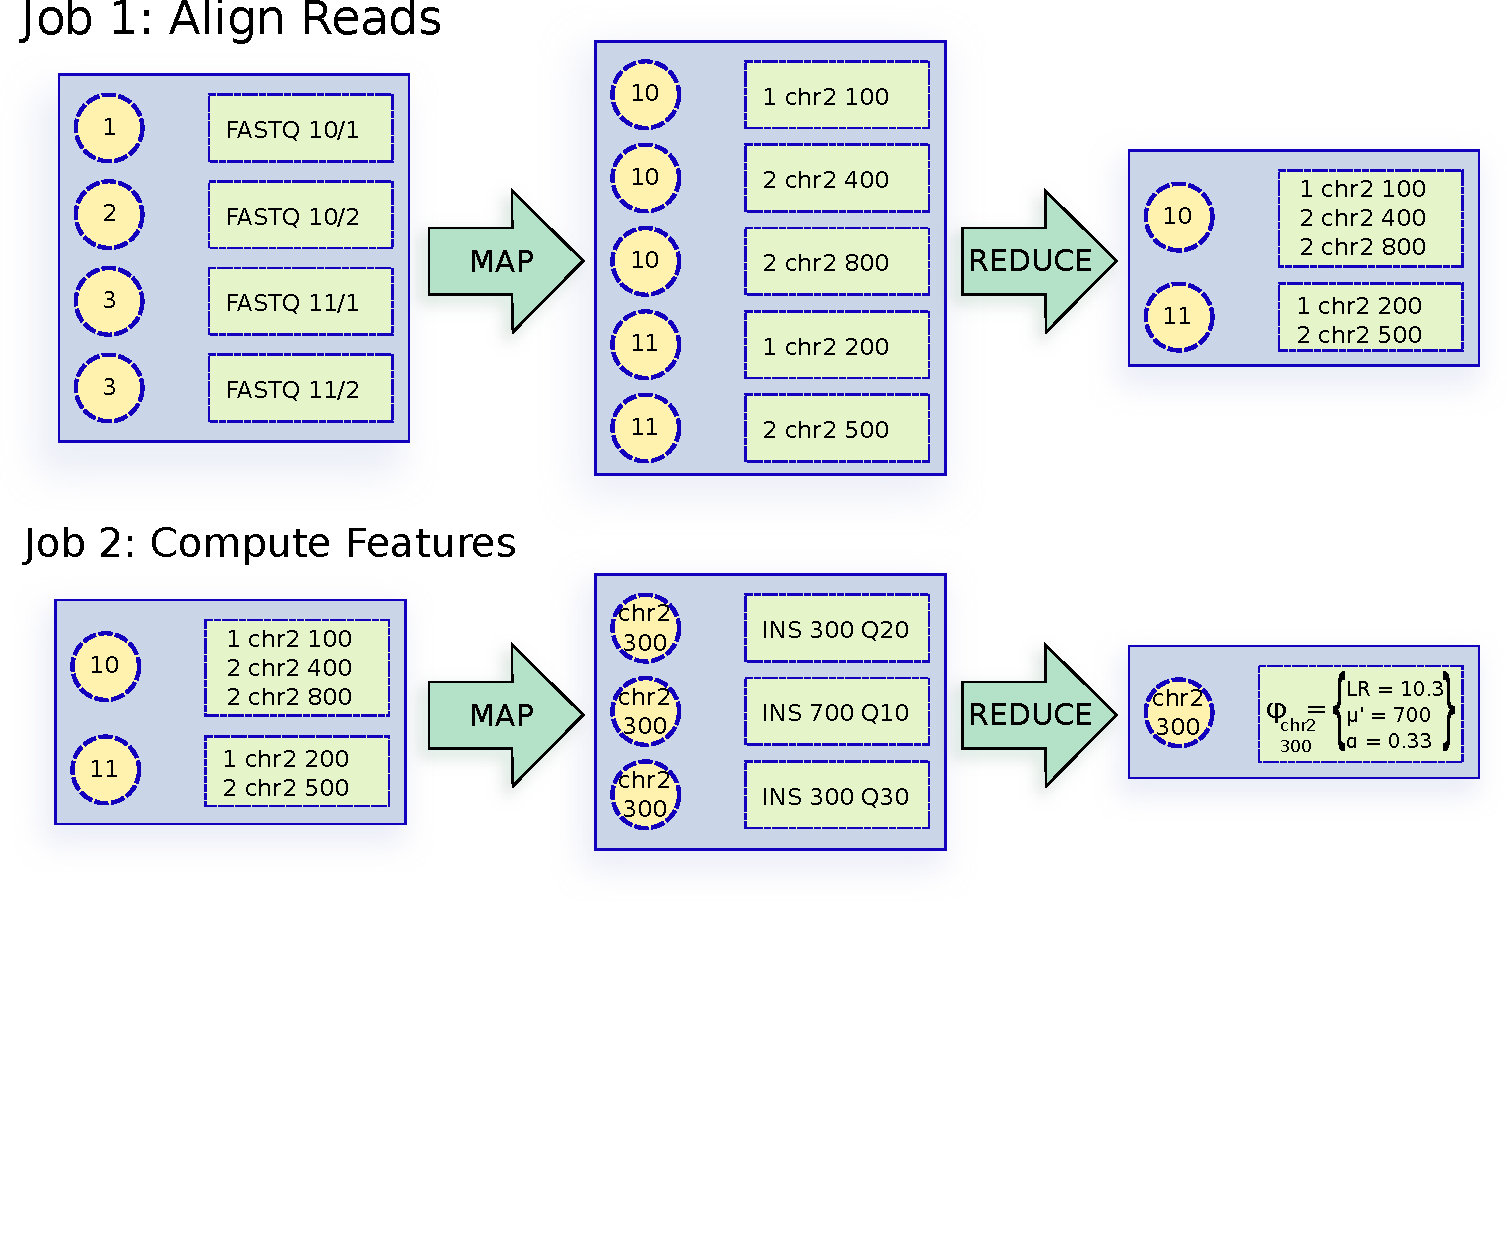
\includegraphics[width=\textwidth,height=0.8\textheight,keepaspectratio]{cloudbreak_mapred_diagram_build_2.pdf}
  \end{center}
\end{frame}

% 8 Algo part 3 - SV calls
\begin{frame}{Cloudbreak Algorithm Job 3: Call SVs}
  \begin{center}   
    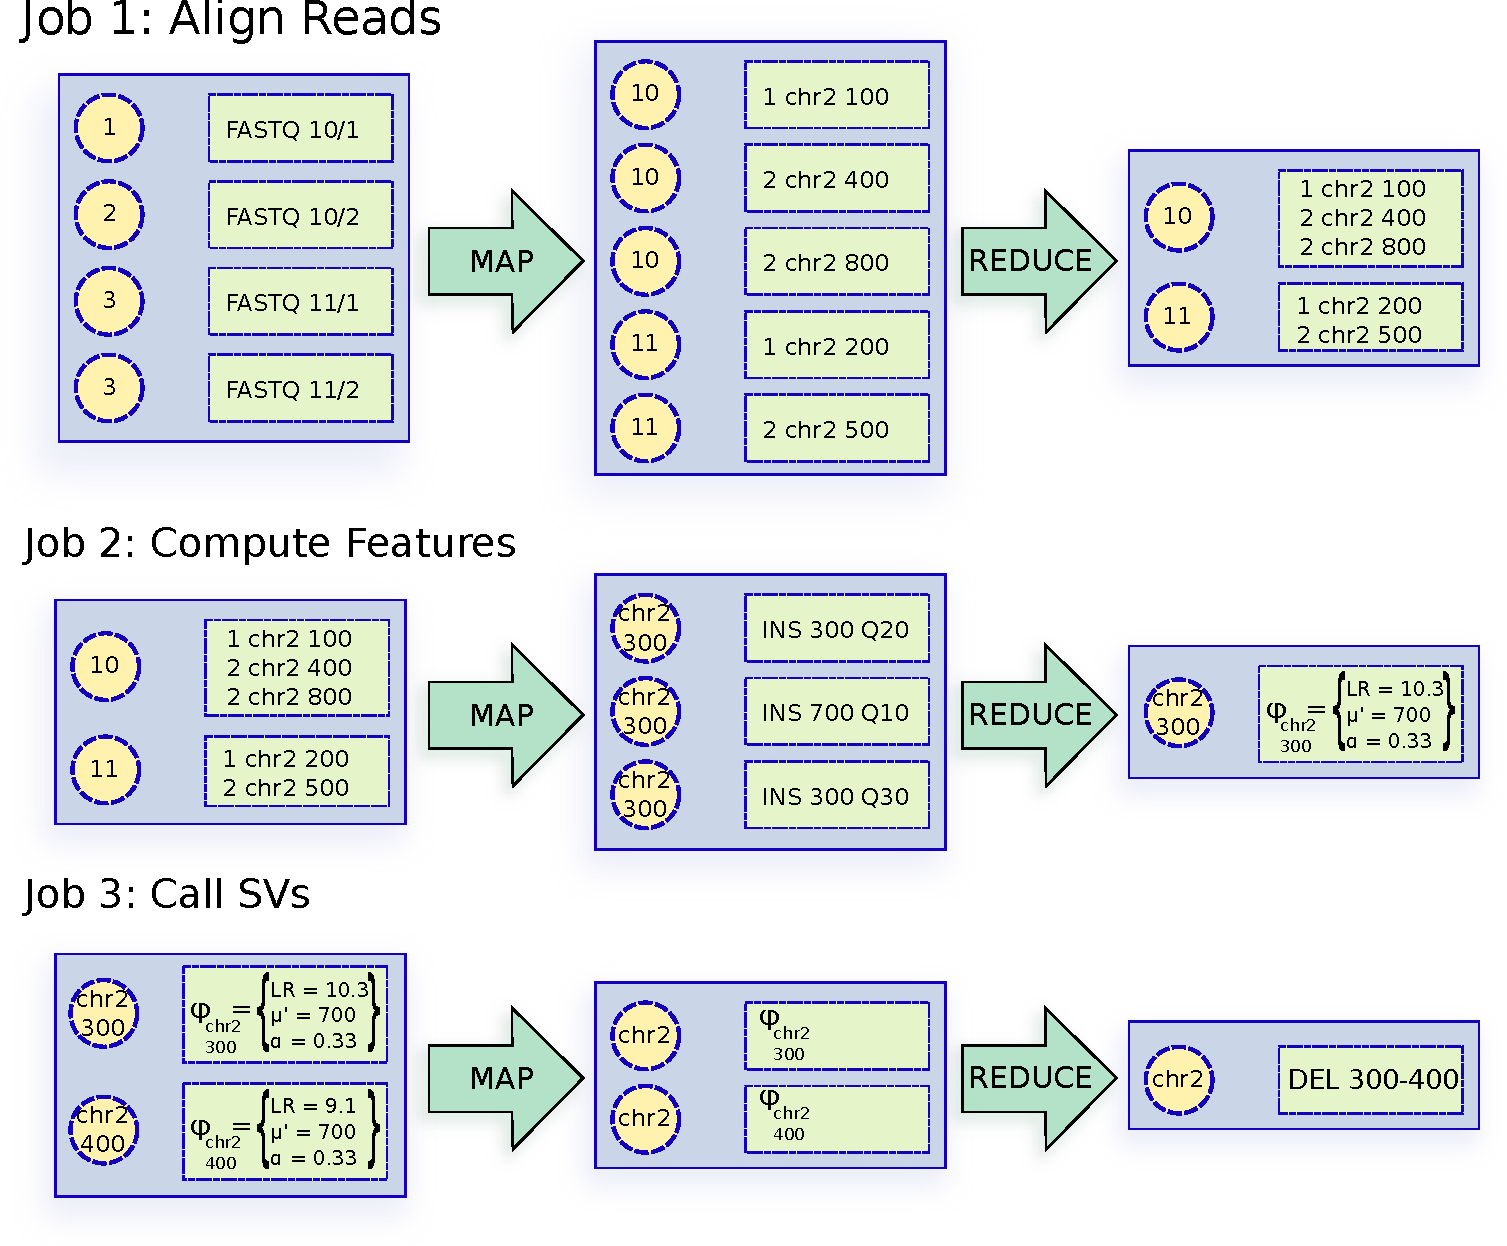
\includegraphics[width=\textwidth,height=0.8\textheight,keepaspectratio]{cloudbreak_mapred_diagram_build_3.pdf}
  \end{center}
\end{frame}

% 10 Evaluation setup
% \begin{frame}
%   \frametitle{Results Comparison}
%   \begin{itemize}
%   \item We compare Cloudbreak to a selection of widely used
%     algorithms taking different approaches:
%   \item Breakdancer (Chen et al. 2009): Traditional RP based approach
%   \item DELLY (Rausch et al. 2012): RP based approach with SR
%     refinement of calls
%   \item GASVPro (Sindi et al. 2012): RP based approach, uses ambiguous
%     mappings of discordant read pairs which it resolves through MCMC
%     algorithm; looks for RD signals at predicted breakpoint locations
%     by examining concordant pairs
%   \item Pindel (Ye et al. 2009): SR approach; looks for clusters of read pairs
%     where only one read could be mapped and searches for split read
%     mappings for the other read
%   \item MoDIL (Lee et al. 2009): Mixture of distributions; only on
%     simulated data due to runtime requirements.
%   \end{itemize}
% \end{frame}

% \begin{frame}
%   \frametitle{Simulated Data}
%   \begin{itemize}
%   \item Very little publicly available NGS data from a genome with fully characterized structural variations
%   \item Can match algorithm output to validated SVs, but don’t know if novel predictions are wrong or undiscovered.
%   \item Way to get a simulated data set with ground truth known and
%     realistic events: take a (somewhat) fully characterized genome,
%     apply variants to reference sequence, simulate reads from modified
%     reference.
%   \item Use Venter genome (Levy et al, 2007), chromosome
%     2.
%   \item To simulate heterozygosity, randomly assign half of the
%     variants to be homozygous and half heterozygous, and create two
%     modified references.
%   \item Simulated 100bp paired reads with a 100bp insert size to 30X coverage.
%   \end{itemize}
% \end{frame}

% \begin{frame}
%   \frametitle{NA18507 Data Set}
%   \begin{itemize}
%   \item Well studied sample from a Yoruban male individual
%   \item High quality sequence to 37X coverage, 100bp reads with a
%     100bp insert size
%   \item We created a gold standard set of deletions from three
%     different studies with low false discovery rates: Mills et
%     al. 2011, Human Genome Structural Variation Project (Kidd et
%     al. 2008), and the 1000 Genomes Project (Mills et al. 2011)
%   \end{itemize}
% \end{frame}

\begin{frame}{Evaluation}
\begin{itemize}
\item Simulated data
\begin{itemize}
\item Indels from the HuRef genome applied to chr2 reference
\item Diploid
\item 30X, 100bp reads, 100bp internal insert size
\end{itemize}
\item Real data from NA18507
\begin{itemize}
\item 37X, 100bp reads, 112bp internal insert size
\item Gold standard set with merged calls from 1000 Genomes Project, Mills et al. (2011b), Kidd
  et al. (2008)
\end{itemize}
\item Matching criteria
\begin{itemize}
\item Overlap with length difference $<$ 300bp
\end{itemize}
\item Comparisons
\begin{itemize}
  \item RP method Breakdancer (Chen et al. 2009)
   \item RP/SR method DELLY (Rausch et al. 2012)
   \item  RP/RD method GASVPro (Sindi et al. 2012)
   \item SR method Pindel (Ye et al. 2009) 
\end{itemize}
\end{itemize}
\end{frame}

% 11 Results 1 (ROC curves for sim)
\begin{frame}{ROC Curves for Chromosome 2 Simulation}
\begin{center}
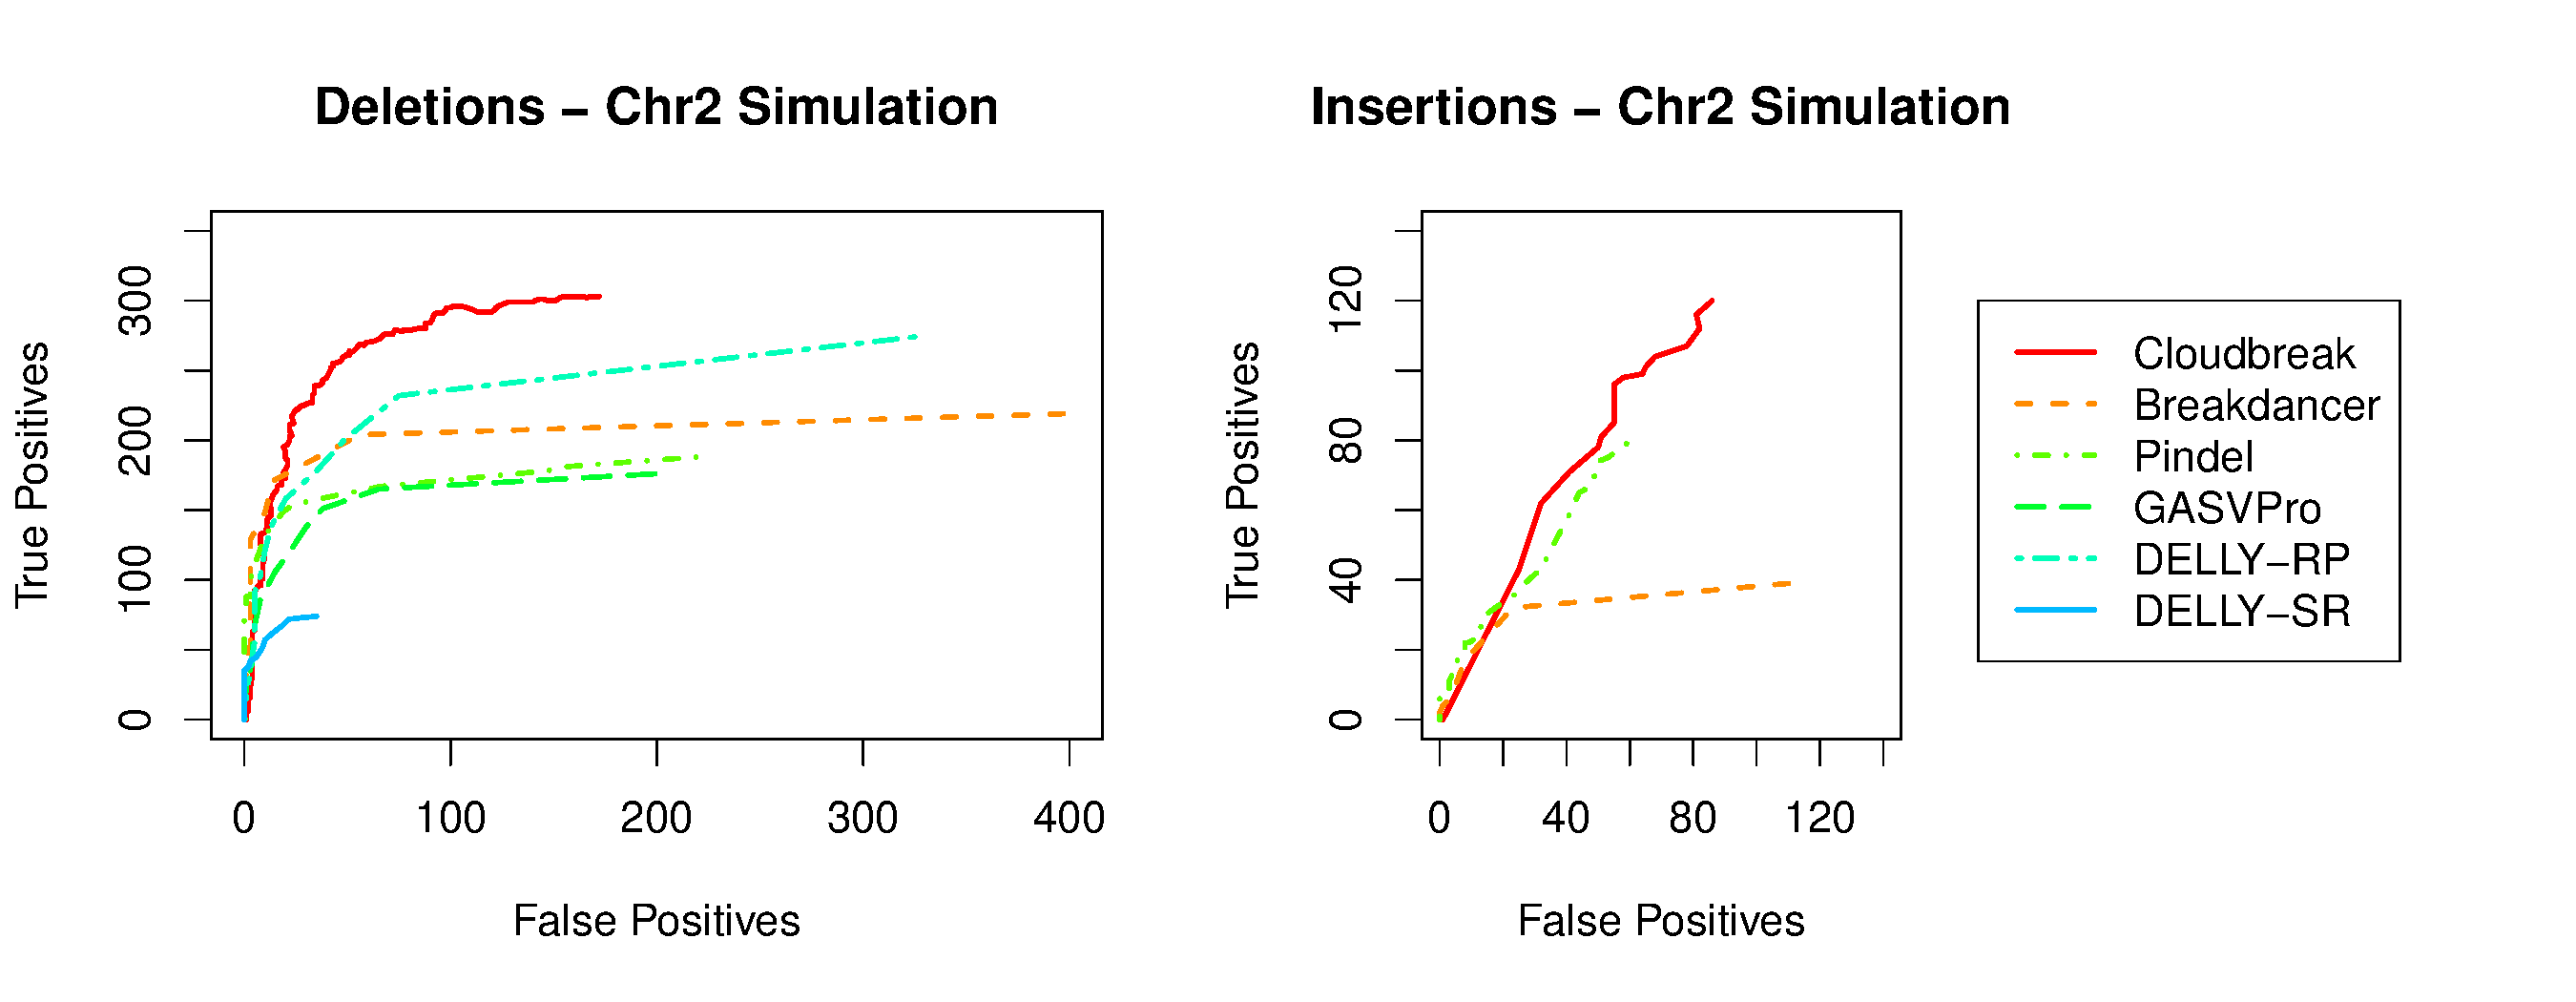
\includegraphics[trim=0 25 0 25, clip, width=1\textwidth]{CHR2SIM_ROC_COMBINED_ROCS_POSTER.pdf}
\end{center}
\begin{itemize}
  \item Caveat: Methods perform better on simulated data than on real
    whole genome datasets.
\end{itemize}
\end{frame}

\begin{frame}{Ability to find simulated variants at a controlled FDR}
\begin{itemize}
\item The number of simulated deletions found by each tool at a 10\% FDR, as well as the number of those deletions that were discovered exclusively by each tool (in parentheses).
\end{itemize}
\begin{center}
\fontsize{7.5pt}{10}\selectfont
\begin{tabular}{rrrrrr}
  \hline
 & 40-100bp  & 101-250bp  & 251-500bp & 501-1000bp & $>$ 1000bp \\ 
 Total Number & 224 &  84 & 82 &  31 & 26\\ 
  \hline
  Cloudbreak  & \textbf{68} (17)  & \textbf{67} (\textbf{10}) &  \textbf{56} (\textbf{5}) & \textbf{11} (\textbf{3}) & \textbf{15} (\textbf{0}) \\ 
  Breakdancer & 52 (8)  & 49 (2) &  49 (0) & 7 (0) & 14 (\textbf{0}) \\ 
  GASVPro     & 35 (2)  & 26 (0) &  26 (0) & 2 (0) & 6 (\textbf{0}) \\ 
  DELLY-RP       & 22 (1)  & 56 (1) &  40 (0) & 8 (0) & 12 (\textbf{0}) \\ 
  DELLY-SR       & 0 (0)  & 2 (0) &  28 (0) & 2 (0) & 10 (\textbf{0}) \\ 
  Pindel      & 60 (\textbf{32})  & 16 (0) &  41 (2) & 1 (0) & 12 (\textbf{0})\\ 
   \hline
\end{tabular}
\end{center}
\end{frame}

%12 Results 2 (ROC curves for NA18507)
\begin{frame}{ROC Curves for NA18507}
\begin{center}
  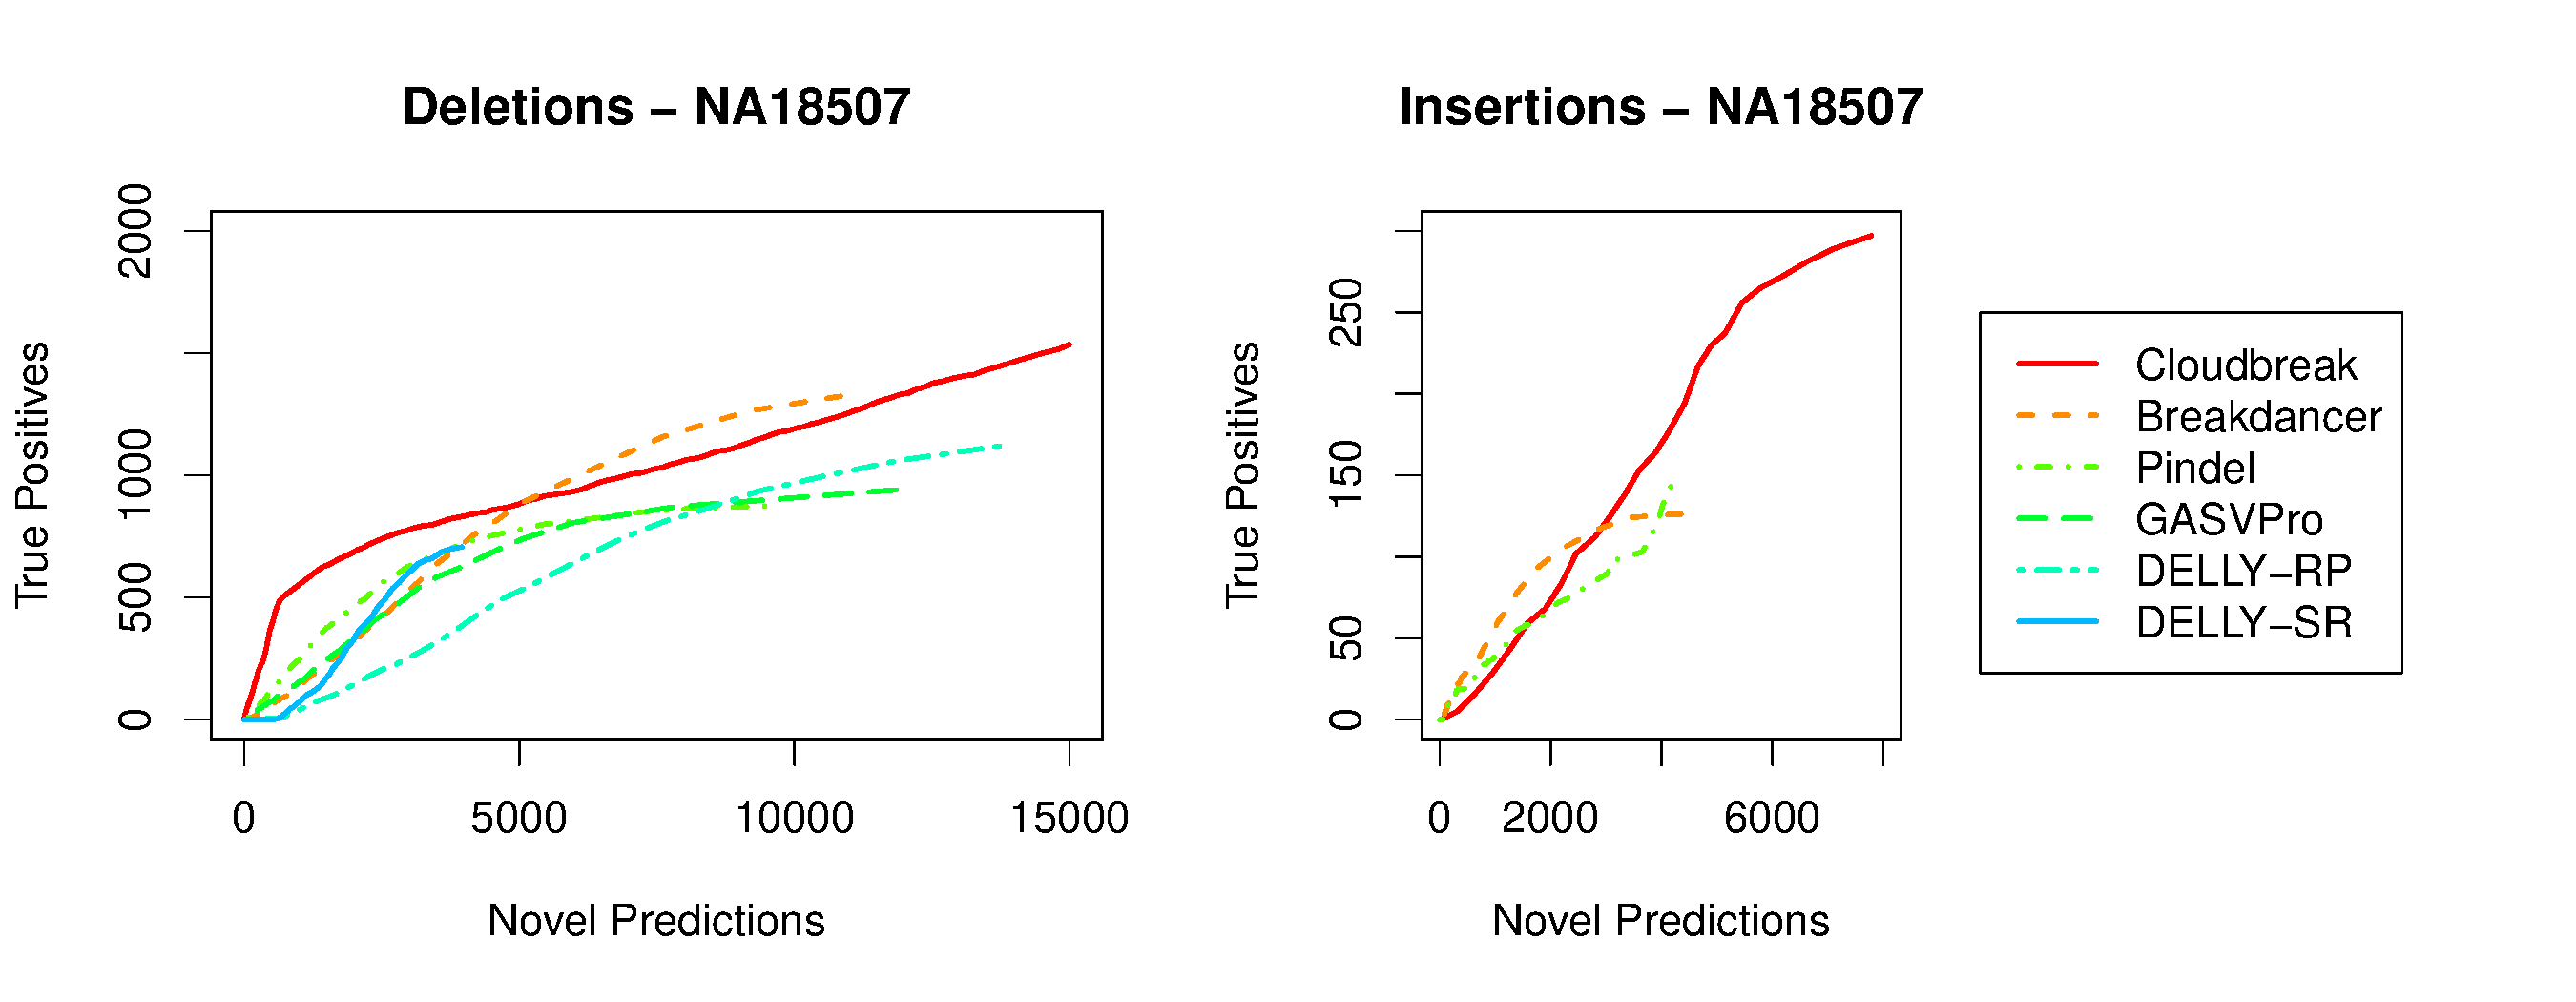
\includegraphics[trim=0 25 0 25, clip, width=1\textwidth]{NA18507_COMBINED_ROCS_POSTER.pdf}
\end{center}
\end{frame}

\begin{frame}
  \frametitle{Run Times}
\begin{center}
  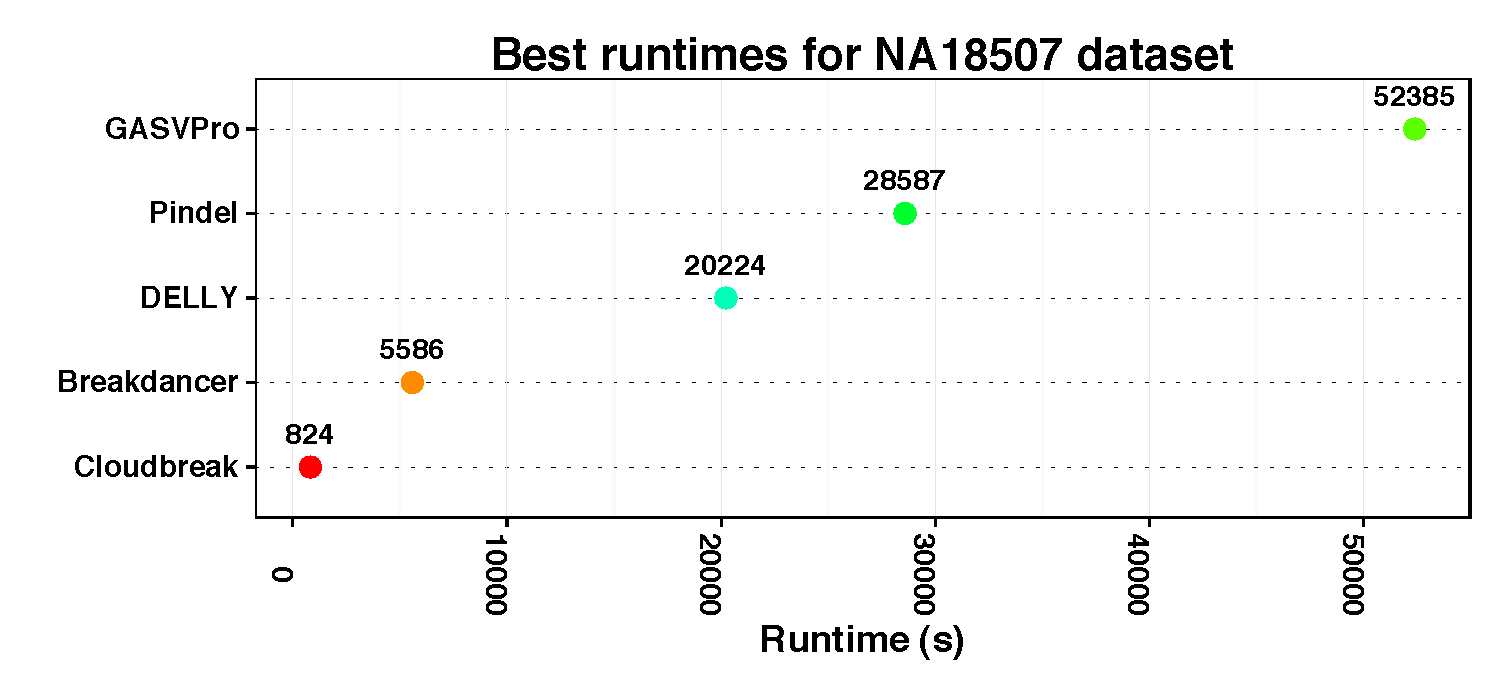
\includegraphics[width=.75\textwidth]{NA18507BestRuntimes_horizontal.pdf}
\end{center}
\fontsize{7.5pt}{10}\selectfont
\begin{center}
\begin{tabular}{r|r|rrr|rrr}
\multicolumn{2}{c}{}  & \multicolumn{3}{c}{Simulated Data} & \multicolumn{3}{c}{NA18507} \\
\hline
 & SV Types &  Single CPU & Parallel & Proc. &  Single CPU & Parallel & Proc.  \\ 
  \hline
  Cloudbreak & D,I &   NA    & 290 & 312    & NA         & 824 & 636 \\ 
  Breakdancer & D,I,V,T &  653   & NA       & NA          & 134,170 &  5,586 & 84 \\
  GASVPro & D,V   &  3,339  & NA       & NA         & 52,385  & NA & NA \\
  DELLY & D         &  1,964 & NA          & NA      & 30,311  & 20,224 & 84 \\
  Pindel & D,I,V,P         & 37,006 &  4,885     & 8          &  284,932  & 28,587 & 84 \\ 
  MoDIL & D,I        &  NA      & 52,547 & 250 & NA         & NA  & NA\\ 
   \hline
\end{tabular}
\\
SV Types - D: Deletions; I: Insertions; V: Inversions; T:
Translocations; P: Duplications \\
All times in seconds 
\end{center}
  \end{frame}



%15 Results 5 (Runtimes)

\begin{frame}{Automatic provisioning of clusters in the cloud}
\begin{center}
    \only<1>{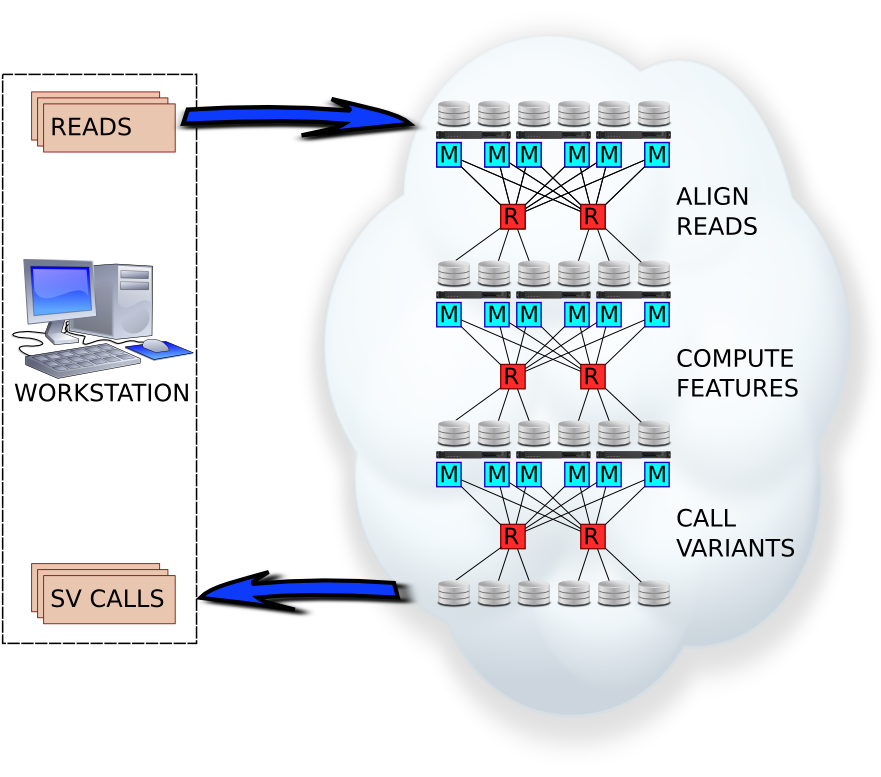
\includegraphics[width=\textwidth,height=0.9\textheight,keepaspectratio]{workflow_with_whirr_build1.png}}
    \only<2>{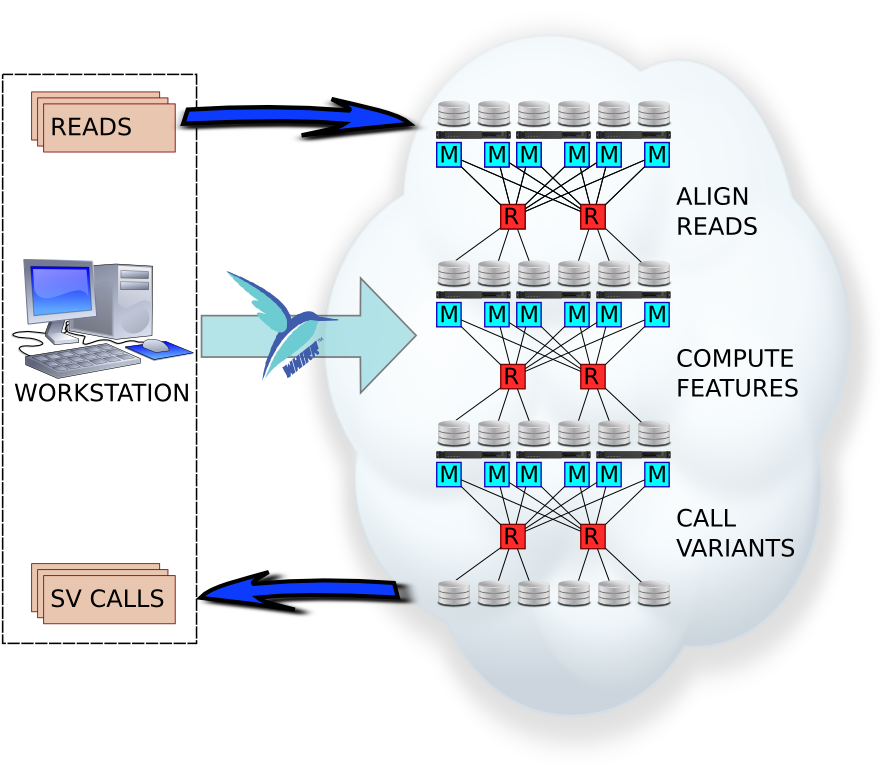
\includegraphics[width=\textwidth,height=0.9\textheight,keepaspectratio]{workflow_with_whirr.png}}
\end{center}
\end{frame}

%17  Discussion/results
\begin{frame}
  \frametitle{Cloudbreak Limitations}
  \begin{itemize}    
    \item Very fast to process once in Hadoop, but importing data takes time
    \item More CPU hours used
    \item Lower breakpoint resolution   
  \end{itemize}
  \begin{center}
  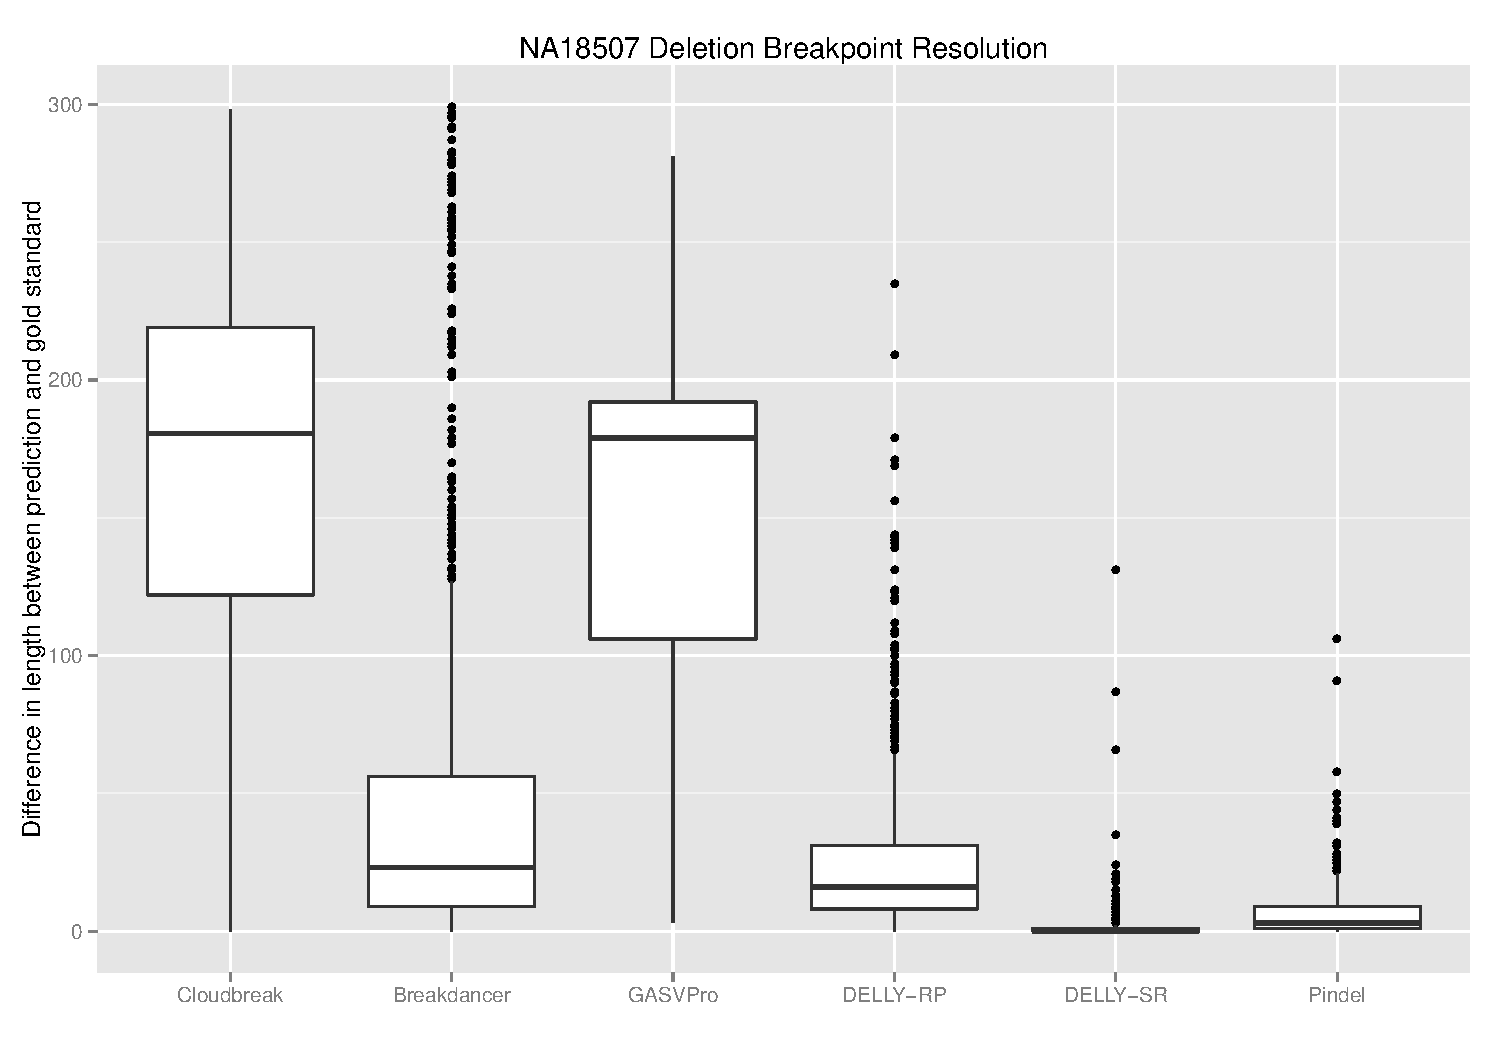
\includegraphics[scale=0.35]{breakpointResolutionNA18507.pdf}
  \end{center}
\end{frame}

\begin{frame}
  \frametitle{Cloudbreak Summary}
  \begin{itemize}
  \item Novel approach to applying MapReduce/Hadoop to the structural
    variation detection problem using the computation of local features
  \item Works for insertions and deletions
    \begin{itemize}
    \item Generalizable to other variant types?
    \end{itemize}
  \item Ability to accurately genotype calls
  \item Greatly decreased runtimes at the cost of more CPU hours
  \item Fast runtimes + accurate region detection but low breakpoint resolution
  \begin{itemize}
    \item Suggests initial scan before
      more in depth \emph{in silico} verification (split read mapping; local assembly;
      discriminative machine learning)
  \end{itemize}
  \item \url{http://github.com/cwhelan/cloudbreak}
  \end{itemize}
\end{frame}

\section{Integrating SV Signals with Discriminative Machine Learning}
\begin{frame}{Outline}
  \tableofcontents[currentsection]
\end{frame}

\begin{frame}{Can Cloudbreak be extended to consider more signals?}
  \begin{itemize}
    \item So far have talked primarily about RP based SV detection
    \item What about other signals? RD, SR, prior knowledge?
    \item Some tools integrate multiple signals, but primarily with \emph{ad hoc} rules:
      \begin{itemize}
        \item DELLY: verify RP predictions with SR mappings
        \item GASVPro: look for RD signals to lend support to RP predictions, e.g. in deletion regions or at inversion breakpoints
        \item Genome STRiP: combine many signals to genotype loci in a population
      \end{itemize}
     \item Cloudbreak's formulation in terms of local features lends itself to integration of signals
  \end{itemize}
\end{frame}

\begin{frame}{Integrating many features in a sequential labeling problem}
  \fontsize{10pt}{10}\selectfont
  \begin{itemize}
    \item For Cloudbreak, we formulated the problem as finding the label of
      each window (i.e. Deletion/No Deletion) based on window features
    \item Let labels be $Y_1,Y_2,...,Y_n$ and feature observations be $X_1,X_2,...,X_n$
   \begin{overlayarea}{.9\textwidth}{.4\textheight}
    \only<1>{
          \item Should be able to model sequential relationship of labels...
    }
    \only<2>{  
    \item Could use a Hidden Markov Model
    \begin{itemize}
      \item Models the joint probability of labels and observations: $P(X,Y)$.
      \item One problem: nearby features might be highly correlated, but HMM assumes that 
        $P(X_i|Y_1,Y_2,...,Y_i,X_1,X_2,...,X_{i-1}) = P(X_i|Y_{i})$
      \item Another: We are modeling $P(X,Y) = P(Y|X)P(X)$, but we only really care about $P(Y|X)$
    \end{itemize}    
    }
    \only<3>{
      \item Conditional Random Fields
      \begin{itemize}
        \item Undirected graphical model
        \item Labels and observations are related by feature functions, which can
          incorporate data from any of the observations
        \item Can be trained to learn $P(Y|X)$ directly (discriminative)      
      \end{itemize}
    }
  \end{overlayarea}
  \end{itemize}
  \begin{center}
%  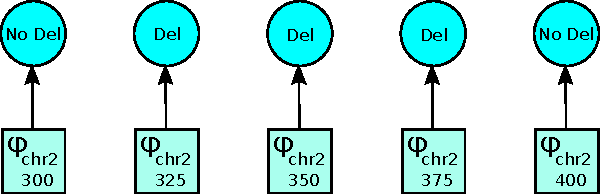
\includegraphics[height=0.4\textheight,keepaspectratio]{graphical-model-0.pdf}
 \multiinclude[<+>][format=pdf,graphics={height=0.3\textheight,keepaspectratio}]{graphical-model}
  \end{center}
\end{frame}

\begin{frame}{CRF Features}
  \begin{itemize}
  \item Insert sizes (RP)
    \begin{itemize}
      \item GMM Features from Cloudbreak (likelihood ratio, $\mu'$, $\alpha$)
      \item Sliding window change point detection      
\vspace{.5mm}
  \def\svgwidth{.75\textwidth}
        \input{segment_change_point.pdf_tex}
    \end{itemize}
  \item Depth and depth changes (RD)
    \begin{itemize}
      \item Average depth of coverage by reads in window
      \item Coverage change points
      \item Sharp drops in coverage from surrounding neighborhood
    \end{itemize}
  \item Split-Read (SR) related signals
    \begin{itemize}
      \item \emph{Soft clipped} mappings 
      \item Singleton mappings
    \end{itemize}
  \item Genome annotations
    \begin{itemize}
      \item Segmental duplications
      \item Annotated repeats and simple repeats
    \end{itemize}
  \end{itemize}
\end{frame}

\begin{frame}{CRF Features}
  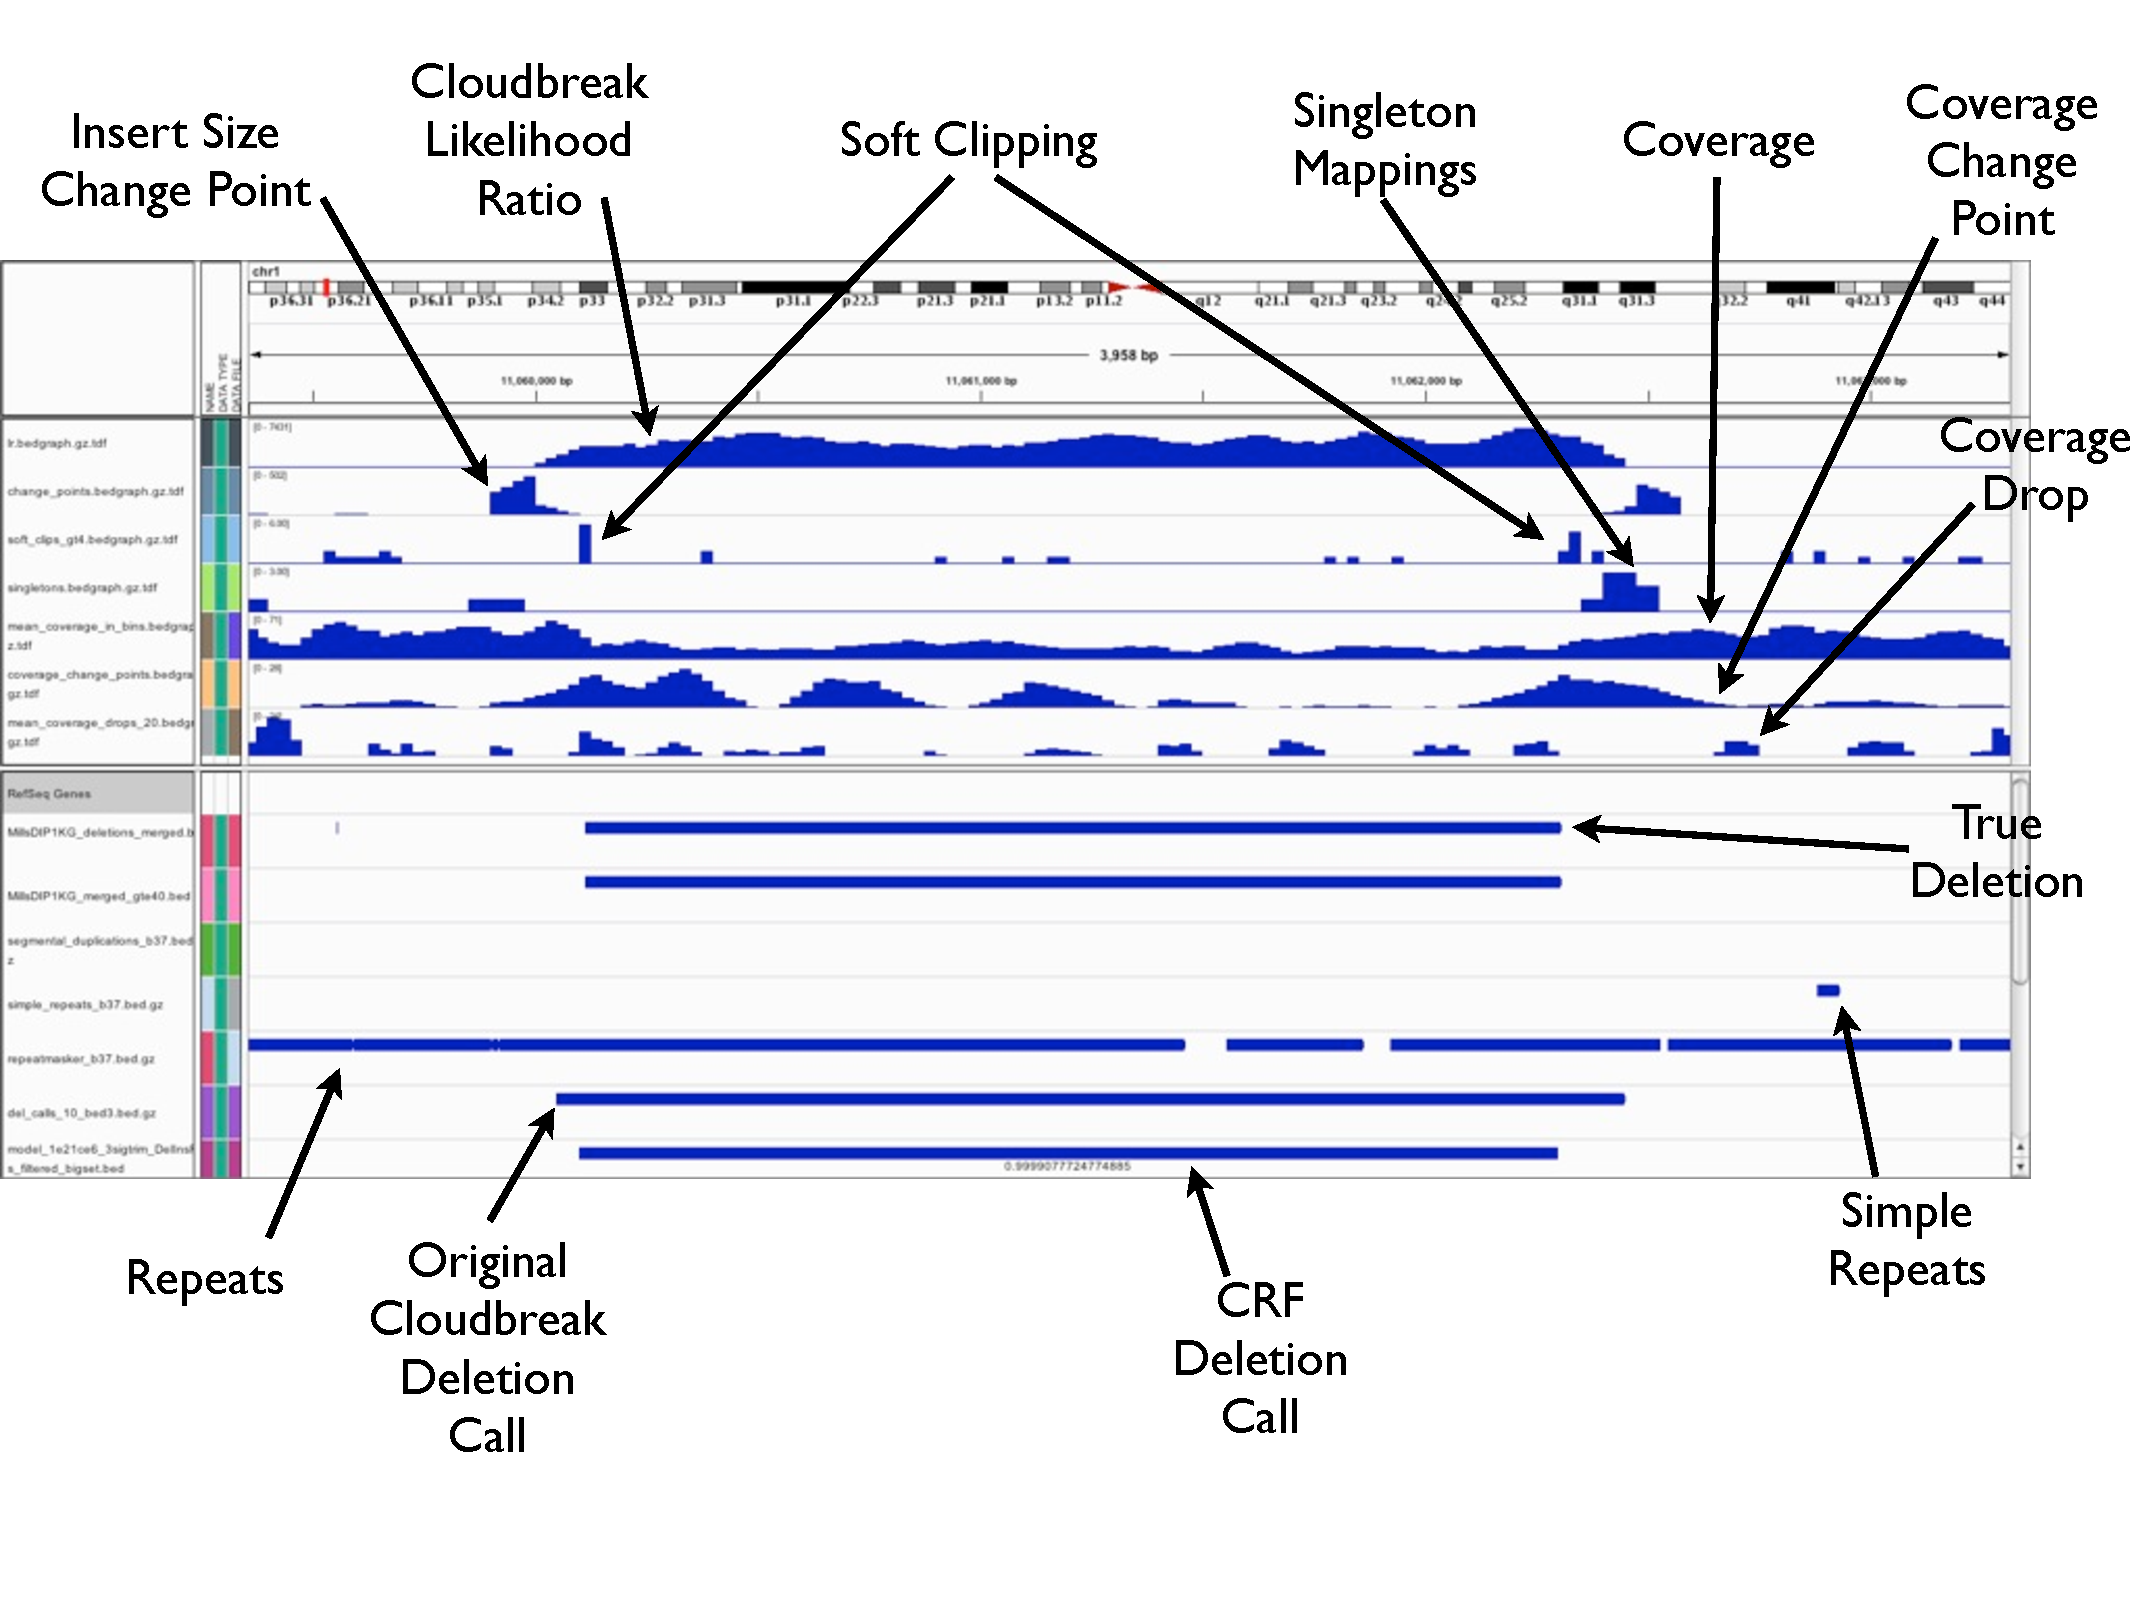
\includegraphics[height=0.9\textheight,keepaspectratio]{true_example_with_features.pdf}
\end{frame}

\begin{frame}{CRF Strategy}
  \begin{itemize}
    \item Label training data \\
\vspace{1mm}
  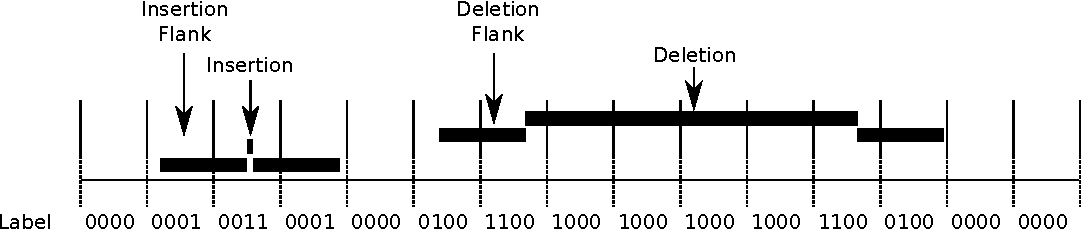
\includegraphics[width=0.8\textwidth,keepaspectratio]{crf_labelling.pdf}

    \item Train CRF on data from simulated variant genome
    \begin{itemize}
      \item All insertions and deletions
      \item False positive calls from Cloudbreak
    \end {itemize}
    \item CRF development in Scala using the Factorie library
    \begin{itemize}
      \item LGBFS optimizer with $L_2$ regularization
    \end{itemize}
    \item Use CRF calls to refine Cloudbreak predictions, adjust score
    \item Test on NA18507 data set with the same gold standard
  \end{itemize}
\end{frame}

\begin{frame}{CRF Results}
 Very modest accuracy improvement
 \begin{center}
   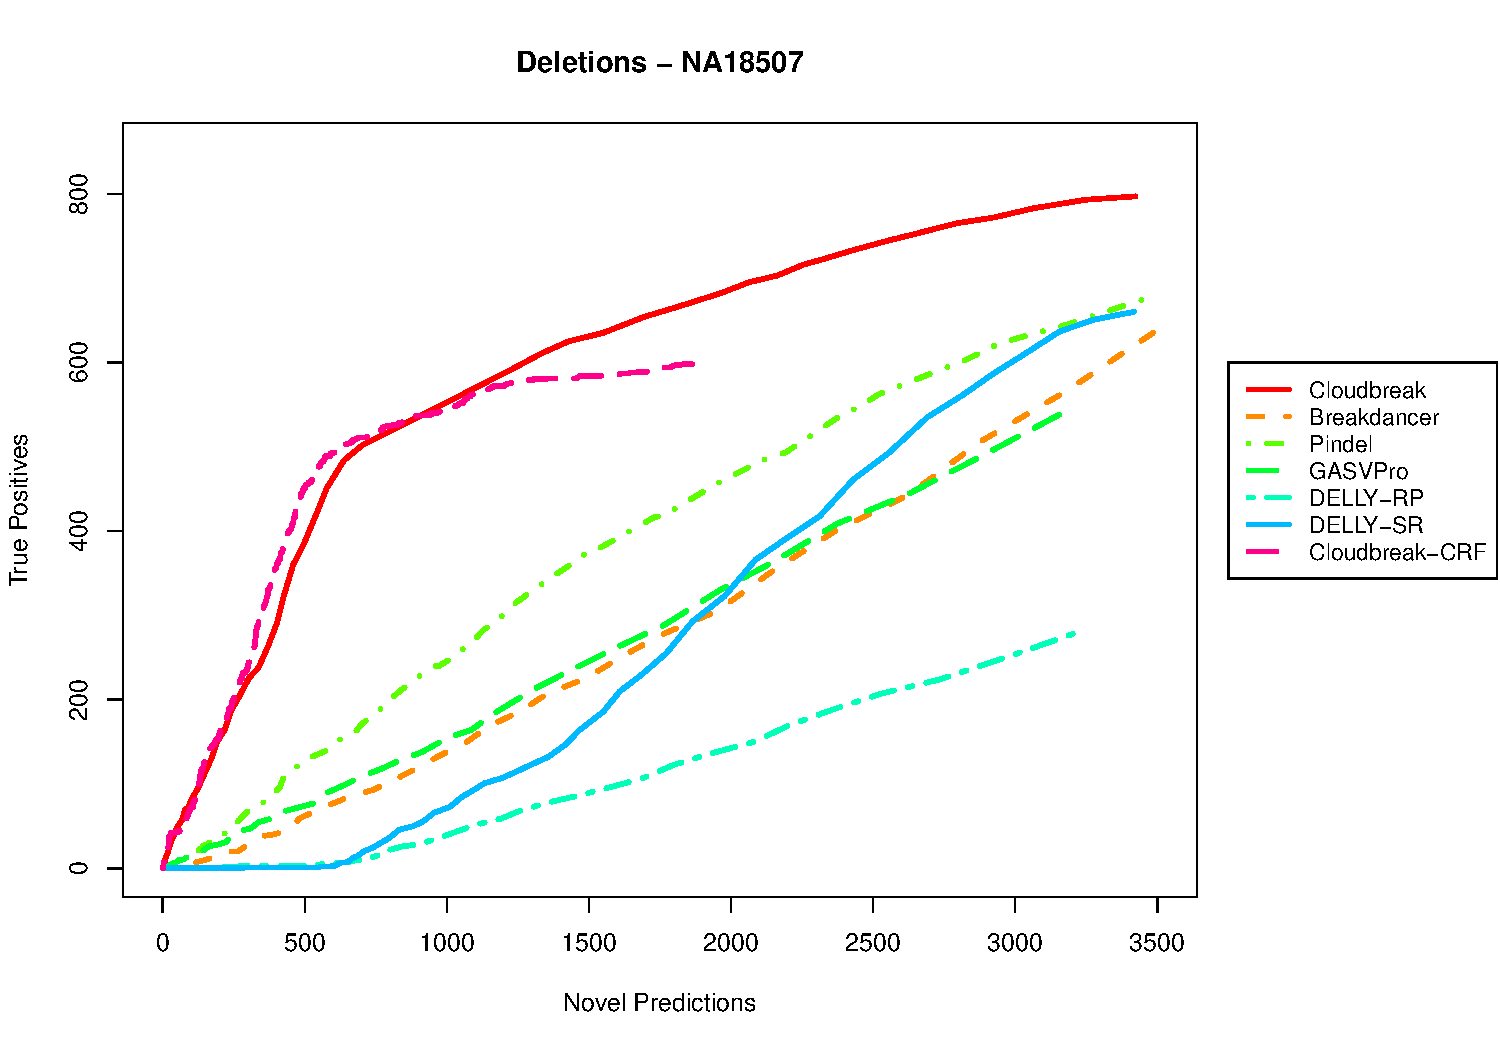
\includegraphics[height=.8\textheight,keepaspectratio]{NA18507_DELS_ROC_with_CRF.pdf}
 \end{center}
\end{frame}

\begin{frame}{CRF Results}
 Good improvement in breakpoint resolution
 \begin{center}
   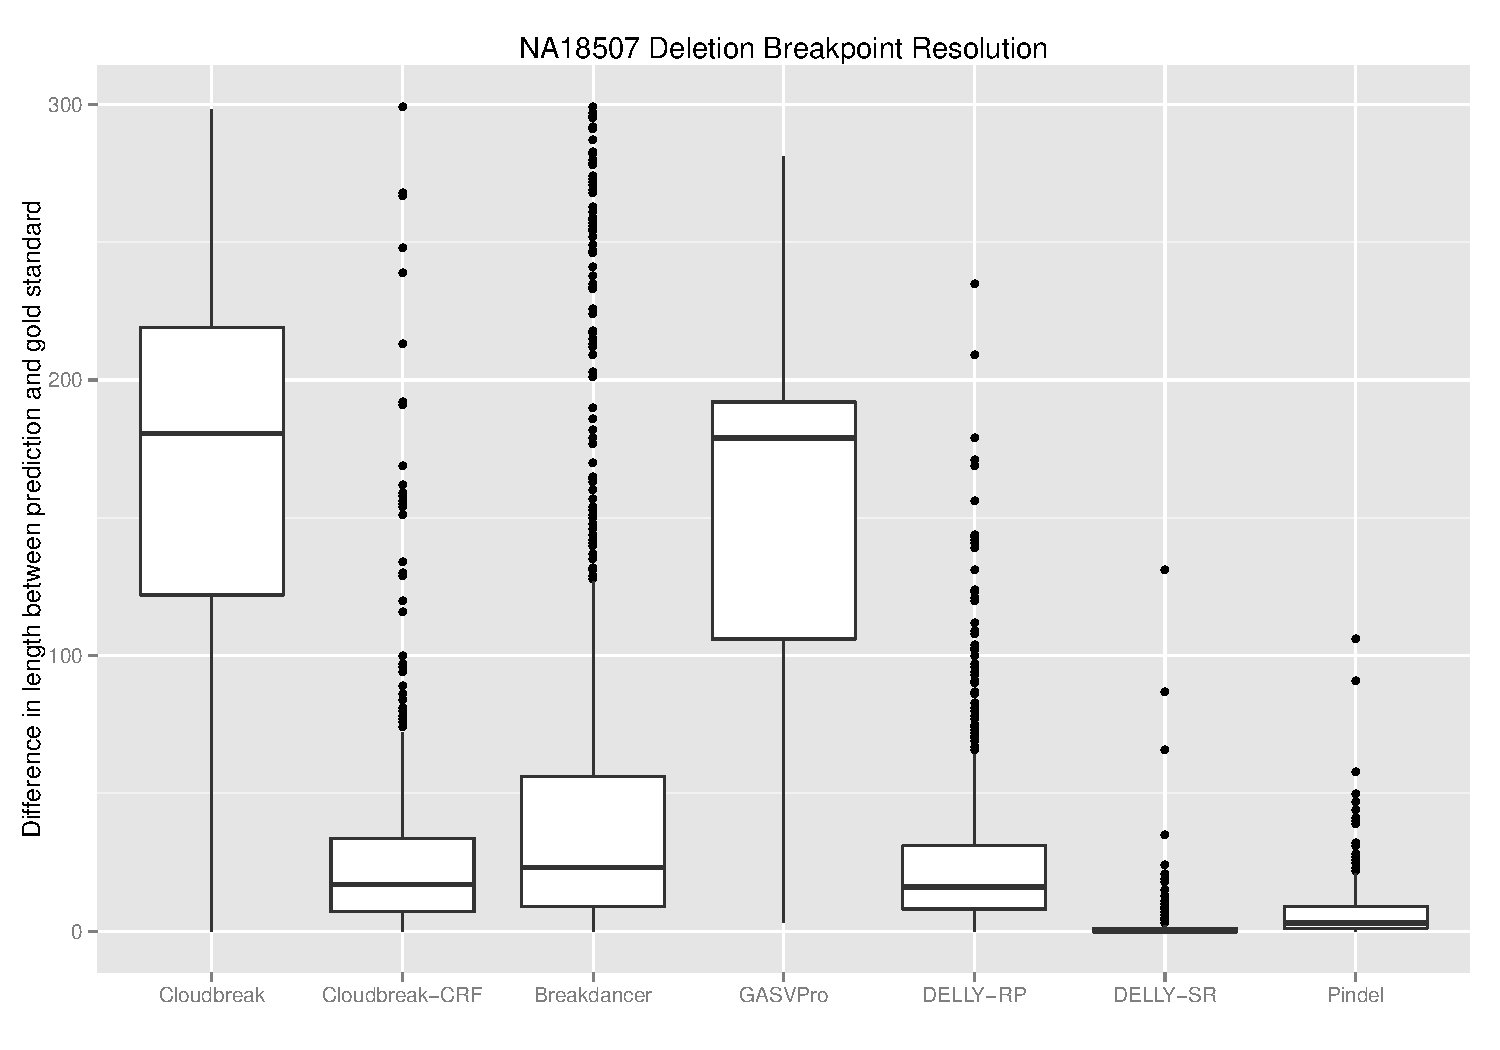
\includegraphics[height=.7\textheight,keepaspectratio]{breakpointResolutionNA18507_withCRF.pdf}
 \end{center}
\end{frame}

\section{Discussion}
\begin{frame}{Outline}
  \tableofcontents[currentsection]
\end{frame}

\begin{frame}{Summary}
  \begin{itemize}
    \item Developed a SV detection algorithm for small deletions and insertions that:
      \begin{itemize}
        \item Reformulates the problem in terms of local features
        \item Has good accuracy
        \item Runs very fast on large clusters
        \item Has the scalability of Hadoop/MapReduce
      \end{itemize}
    \item Described a method for integrating multiple signals of structural variation that:
      \begin{itemize}
        \item Uses discriminative machine learning
        \item Improves breakpoint resolution
        \item Could be extended to incorporate a wide variety of features
       \end{itemize}
   \end{itemize}
\end{frame}

\begin{frame}{Future work}
  \begin{itemize}
    \item Detect other variant types (inversions, MEIs)
    \item Integrate with other components to create a scalable end-to-end Hadoop genomics pipeline
    \item Apply ideas from Cloudbreak to population-scale SV callers (Genome STRiP)
    \item Feature computation algorithms for non diploid or heterogeneous samples (tumors)
    \item More complete training and testing sets for discriminative machine learning approaches
    \item Other machine learning techniques - deep learning
  \end{itemize}
\end{frame}

\begin{frame}{What could we do with scalable and accurate SV calling?}
  \begin{itemize}
    \item Map how structural variation interacts with coding and 
      regulatory elements across the genome
      \begin{center}
      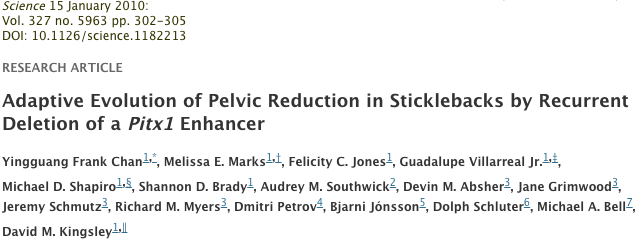
\includegraphics[width=.6\textwidth]{stickleback_paper.png}
      \end{center}
    \item Improve understanding of how genomic and epigenetic features interact
      with structural variants
      \begin{itemize}
        \item Insights from gibbon genome?
      \end{itemize}
    \item Enable incorporation of structural variants into clinical genomic pipelines
  \end{itemize}
\end{frame}

\begin{frame}{Acknowledgments}
  Kemal S\"onmez (co-advisor), Lucia Carbone (co-advisor), Izhak Shafran
 \begin{center}
   
\includegraphics[width=.2\textwidth]{kemal3.jpg} \hspace{20 mm}   
   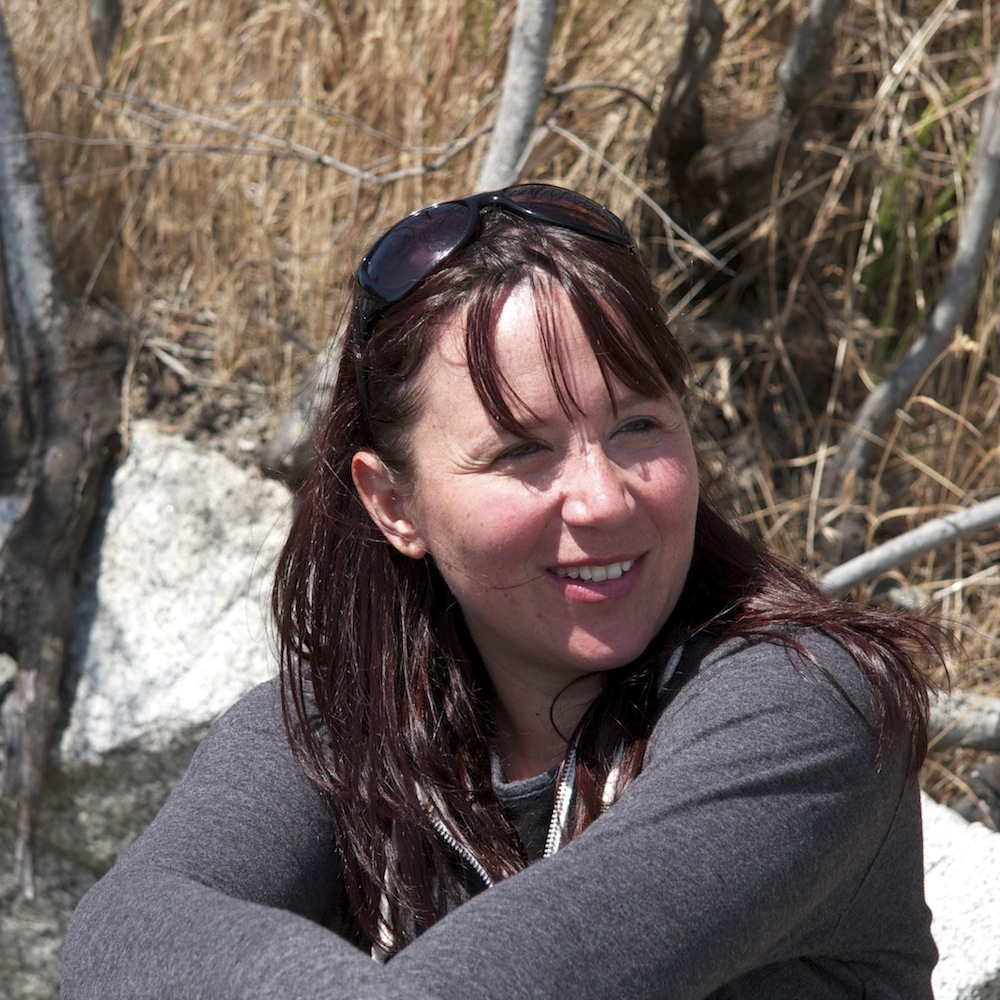
\includegraphics[width=.2\textwidth]{Lucia_Profile.jpg} \hspace{20 mm}
   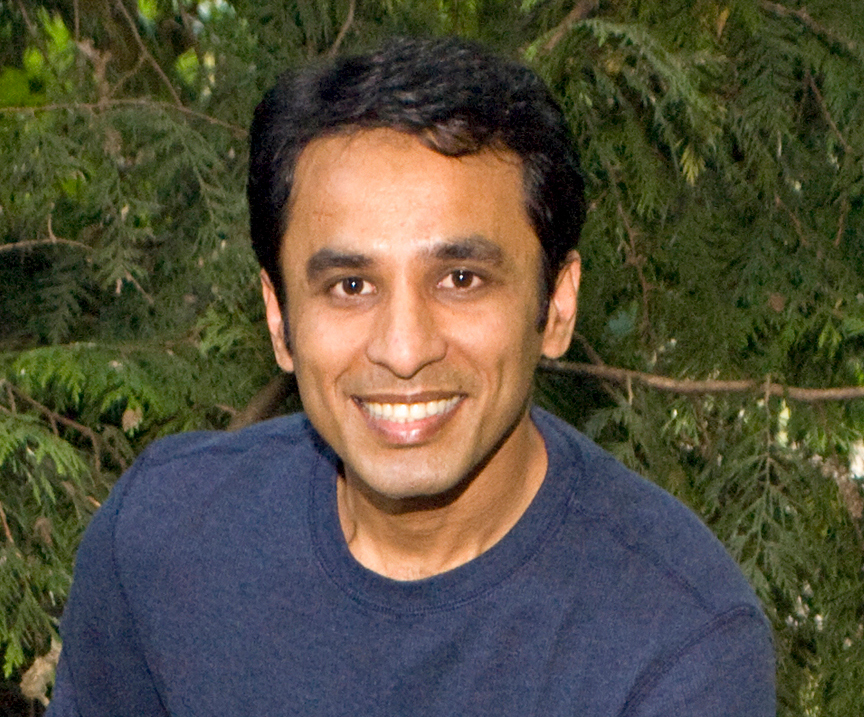
\includegraphics[width=.2\textwidth]{izhak_shafran.jpg}
  \end{center}
  Carbone Lab: Josh Meyer, Larry Wilhelm, Nathan Lazar, Liz Terhune, Kim Nevonen, Eisa Mahyari \\
\vspace{10 mm}
  OHSU Center for Spoken Language Understanding
\end{frame}

\appendix
\newcounter{finalframe}
\setcounter{finalframe}{\value{framenumber}}

\begin{frame}{Ability to find simulated variants at maximum sensitivity}
\begin{itemize}
\item Number of variants found in each size class (number of
  exclusive predictions for algorithm in that class)
\end{itemize}
\begin{center}
\fontsize{6pt}{10}\selectfont
\begin{tabular}{r|rrr|rrrrr}
  \cline{2-9}
   &                     & Prec. & Recall & 40-100bp  & 101-250bp  & 251-500bp & 501-1000bp & $>$ 1000bp \\ 
\hline
\multirow{7}{*}{\begin{sideways}Deletions\end{sideways}} & Total Number &          &           & 224 &  84 & 82 &  31 & 26\\ 
  \hline
\cline{2-9}
&  Cloudbreak    &  0.638 & \textbf{0.678} & \textbf{153} (9)  & 61 (0) &  62 (0) & 12 (0) & 15 (0) \\ 
&  BreakDancer   &  0.356 & 0.49 & 89 (0)  & 54 (0) &  53 (0) & 8 (0) & 15 (0) \\ 
&  GASVPro        & 0.146 & 0.432 & 83 (2)  & 32 (0) &  55 (0) & 8 (0) & 15 (0) \\ 
&  DELLY-RP           & 0.457 & 0.613 & 114 (3)  & \textbf{68} (0) &  \textbf{66} (0) & 9 (1) & 17 (0) \\ 
&  DELLY-SR           & \textbf{0.679} & 0.166 & 0 (0)  & 3 (0) &  49 (0) & 6 (0) & 16 (0) \\ 
&  Pindel           & 0.462 & 0.421 & 96 (\textbf{11})  & 24 (0) &  48 (0) & 5 (0) & 15 (0)\\ 
&  MoDIL           & 0.132  & 0.66 & 123 (6)  & 66 (\textbf{3}) &  \textbf{66} (\textbf{11}) & \textbf{17} (\textbf{7}) & \textbf{23} (\textbf{8})\\ 
   \hline
\multirow{5}{*}{\begin{sideways}Insertions\end{sideways}} & Total Number &          &           & 199 &  83 & 79 &  21 & 21\\ 
\cline{2-9}
&  Cloudbreak   &0.451 & \textbf{0.305}  & \textbf{79} (\textbf{32})  & \textbf{32} (\textbf{18}) &  \textbf{11} (8) & 1 (0) & 0 (0) \\ 
&  BreakDancer & 0.262 & 0.0968  & 23 (5)  & 14 (5) &  2 (1) & 0 (0) & 0 (0) \\ 
&  Pindel          & \textbf{0.572} & 0.196 & 52 (25)  & 5 (1) &  10 (\textbf{9}) & \textbf{3} (\textbf{2}) & \textbf{9} (\textbf{9})\\ 
&  MoDIL          & 0.186 & 0.0521 & 14 (1)  & 4 (0) &  1 (0) & 2 (\textbf{2}) & 0 (0)\\ 
\hline
\end{tabular}
\end{center}
\end{frame}


\begin{frame}{Ability to find NA18507 deletions by size}
\begin{itemize}
\item Using the same cutoffs that yielded a 10\% FDR on the simulated
  chromosome 2 data set, adjusted for the difference in coverage from
  30X to 37X. 
\end{itemize}
\fontsize{6pt}{10}\selectfont
\begin{center}
\begin{tabular}{r|rrr|rrrrr}
  \cline{2-9}
&  & Prec. & Recall & 40-100bp & 101-250bp & 251-500bp & 501-1000bp & $>$ 1000bp \\ 
\hline
\multirow{6}{*}{\begin{sideways}Deletions\end{sideways}} & Total Number & & & 7,462 & 240 & 232 & 147 & 540 \\
  \hline
\cline{2-9}
& Cloudbreak & 0.0943 & \textbf{0.17} & \textbf{573} (\textbf{277})  & \textbf{176} (\textbf{30}) &  \textbf{197} (\textbf{18}) & \textbf{121} (\textbf{6}) & \textbf{399} (\textbf{24}) \\ 
& BreakDancer & 0.137 & 0.123 & 261 (29)  & 136 (3) &  178 (0) & 114 (0) & 371 (0) \\  
&  GASVPro & 0.147 & 0.0474 & 120 (21)  & 40 (2) &  85 (0) & 36 (0) & 128 (0) \\ 
&  DELLY-RP & 0.0931 & 0.1 & 143 (6)  & 128 (3) &  167 (1) & 103 (0) & 323 (1) \\ 
&  DELLY-SR & 0.153 & 0.0485 & 0 (0)  & 26 (0) &  123 (0) & 66 (0) & 203 (0) \\ 
&  Pindel & \textbf{0.179} & 0.0748 & 149 (8)  & 61 (0) &  149 (0) & 69 (1) & 217 (0) \\ 
\hline
\multirow{4}{*}{\begin{sideways}Insertions\end{sideways}} & Total Number & & & 536 & 114 & 45 & 1 & 0 \\
\cline{2-9}
& Cloudbreak & 0.0323 & \textbf{0.455} & \textbf{265} (\textbf{104})  & \textbf{49} (\textbf{24}) &  3 (1) & 0 (0)  & 0 (0)  \\ 
& BreakDancer & 0.0281 & 0.181 & 97 (10)  & 27 (5) &  2 (1) & 0 (0) & 0 (0) \\  
&  Pindel & \textbf{0.0387} & 0.239 & 144 (45)  & 14 (7) &  \textbf{7} (\textbf{6}) & \textbf{1} (\textbf{1}) &  0 (0) \\ 
\hline
\end{tabular}
\end{center}
\end{frame}

%14 Results 4 (Genotyping)
\begin{frame}{Genotyping Deletions}
  \begin{itemize}
  \item Use mixing parameter $\alpha$ to predict genotypes. 
   \item Threshold the average value of $\alpha$ in each
     prediction
   \begin{itemize}
    \item 92.7\% accuracy on simulated data
    \item 95.9\% accuracy on NA18507 (for calls with genotypes from Genome STRiP)
   \end{itemize}
  \end{itemize}
\fontsize{7.5pt}{10}\selectfont
\begin{center}
\begin{tabular}{r|r|rr|rr|}
\multicolumn{2}{c}{}  & \multicolumn{4}{c}{Actual Genotypes} \\
\multicolumn{2}{c}{}  & \multicolumn{2}{c}{Simulated Data} & \multicolumn{2}{c}{NA18507} \\
\cline{3-6}
\multicolumn{2}{c|}{} &  Homozygous & Heterozygous & Homozygous & Heterozygous \\ 
\cline{2-6}
\multirow{2}{*}{\shortstack{Predicted \\ Genotypes}} & Homozygous & 35 & 2 &  96 & 21 \\
 & Heterozygous & 0 & 39 &  2 & 448 \\
\cline{2-6}
\end{tabular}
\end{center}
\end{frame}

\begin{frame}{Scalability}
\center
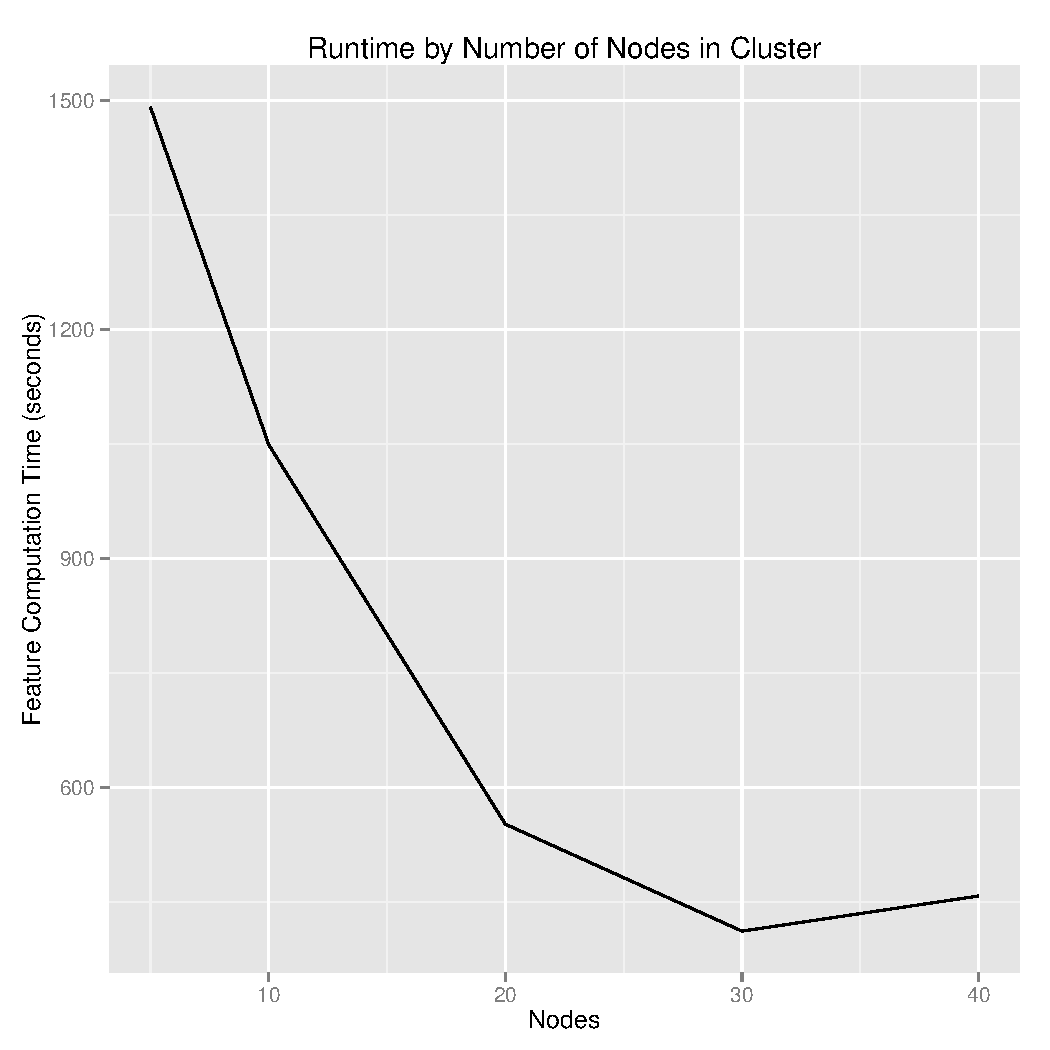
\includegraphics[height=.8\textheight]{runtimeByNodes.pdf}
\end{frame}

\begin{frame}{Effect of Window Size Choice}
\center
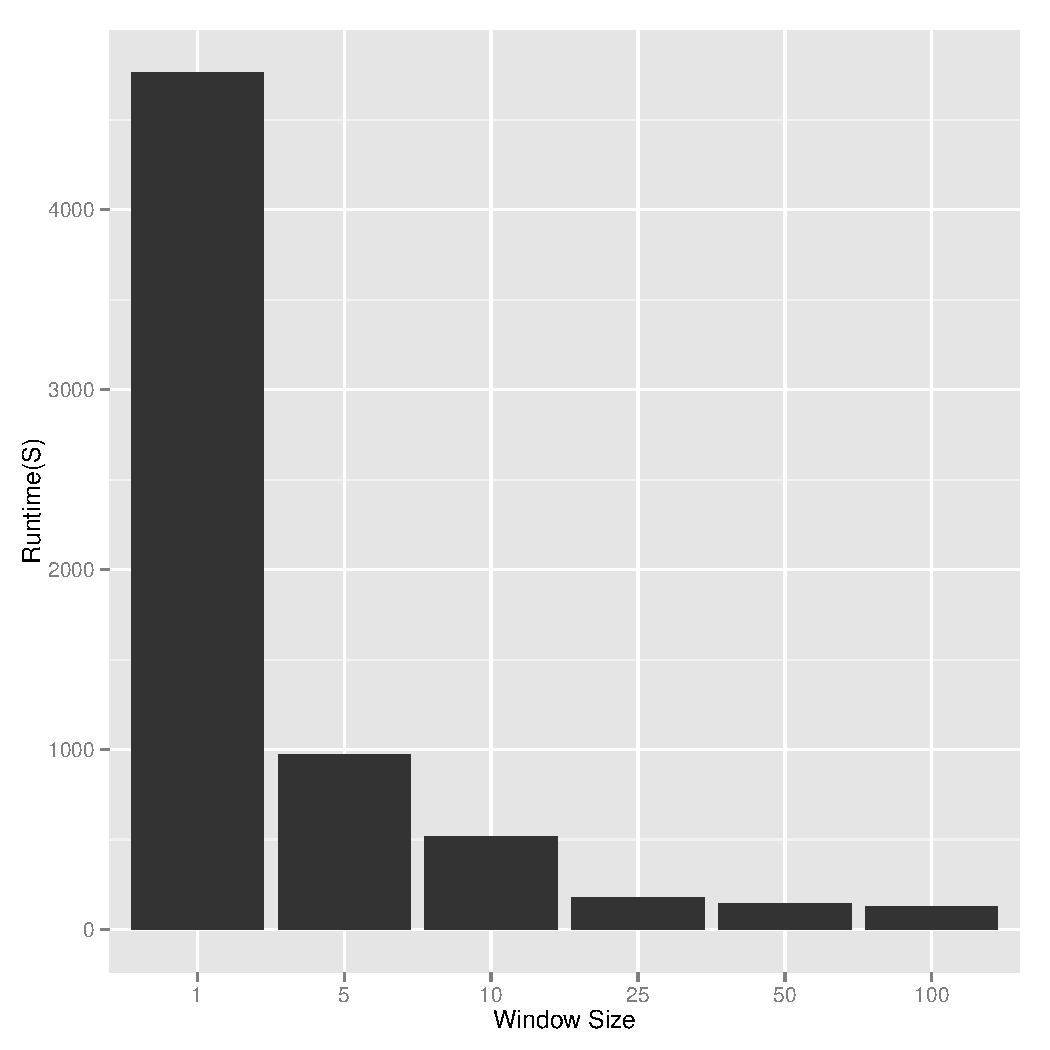
\includegraphics[height=.6\textheight]{runtime_by_windowSize.pdf}\hspace{1mm}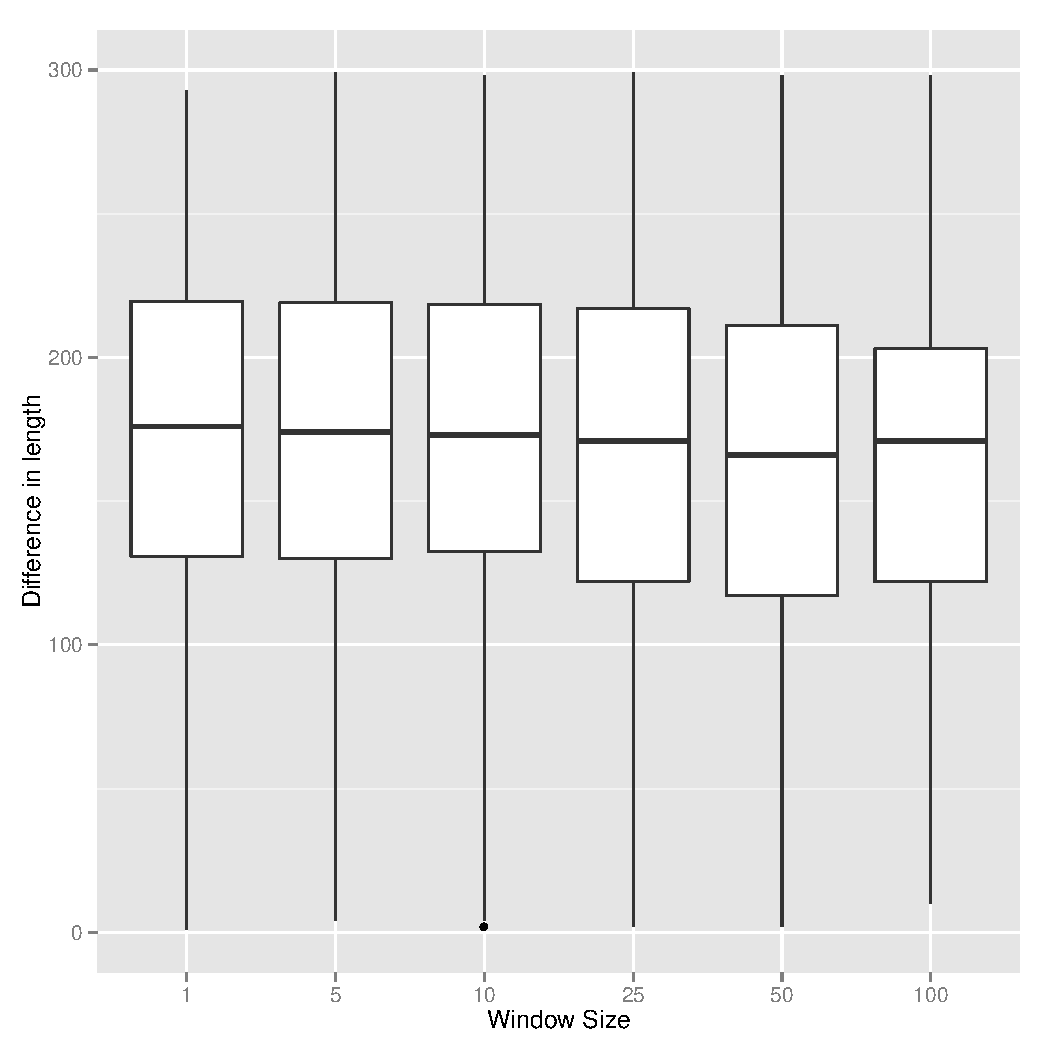
\includegraphics[height=.6\textheight]{breakpoint_resolution_by_windowSize.pdf} \\
\vspace{2mm}
\tiny
\begin{tabular}{r|rrrrr}
 \hline
 Window Size & Calls & True Positives & Precision & Recall & F1 \\ 
 \hline
   1 & 274 & 228 & 0.832 & 0.57 & 0.677 \\ 
   5 & 268 & 228 & 0.851 & 0.57 & 0.683 \\ 
   10 & 258 & 223 & 0.864 & 0.557 & 0.678 \\ 
   25 & 240 & 217 & 0.904 & 0.542 & 0.678 \\ 
   50 & 215 & 194 & 0.902 & 0.485 & 0.631 \\ 
   100 & 162 & 141 & 0.87 & 0.352 & 0.502 \\  
\end{tabular}
\end{frame}

\end{document}
% LocalWords:  textsc ldots ap rp smallskip rpi svs flalign langle rightarrow
% LocalWords:  subseteq mathbb Cloudbreak th Sindi mismappings rrrrrr hline rrr
% LocalWords:  Yoruban rrrrr Prec rr multirow shortstack Rackspace
